\chapter{全球水稻种植区地表降温效应研究}
水稻种植通过改变地表水分条件、植被覆盖和能量交换过程，对地表热状态产生重要影响\cite{Xue2021RemoteSensing,Liu2022AgForMet}。已有研究主要集中于局地或区域尺度，对全球水稻种植区地表温度效应的总体格局、昼夜差异、生长季动态及空间异质性仍缺乏系统认识。%且常以固定月份或区域统一的生长季窗口界定分析时段，
基于 GlobalRice500 数据集提供的逐像元逐日水稻种植区时空分布信息，本章结合 2003--2020 年全球日尺度地表温度数据，以水稻种植区与邻近非水稻耕地在水稻生长季内的地表温度之差量化水稻种植区的温度效应。为提高可比性，选取空间邻近且地形条件相似的非水稻耕地作为对照。% 逐像元水稻分布和逐季生长季边界信息
在此基础上，本章首先分析日间和夜间地表温度效应的全球空间分布、年际稳定性及不同气候区差异；随后考察地表温度效应随十公里网格内水稻种植区比例、水稻种植区规模以及非水稻耕地梯度环带的变化；并进一步基于生长季日序刻画不同水稻种植区规模降温效应的生长季动态。%距水稻种植区边界距离
最后，从地表能量平衡、空间分布特征和不确定性来源等方面，讨论水稻种植区降温效应的形成过程、科学意义与解释边界。

\section{全球水稻种植区地表降温总体评估}
\label{sec:overall_dlst}

为量化水稻种植区的地表温度效应，本节首先界定水稻种植区地表降温效应的比较对象和物理含义，以水稻种植区与非水稻种植区之间的水稻生长季地表温度差异定义水稻种植区地表降温效应量化指标 $\Delta\mathrm{LST}$。
随后，为减弱土地覆盖、局地气候背景和地形条件差异对量化结果的干扰，按照耕地属性一致、空间邻近、高程相近和样本数量充足等条件筛选非水稻耕地对照样本。
考虑到样本的空间聚集性及多年观测之间的时间相关性，进一步采用时空分块自助抽样法（block bootstrap）评估水稻种植区温度效应量化的统计不确定性。
在此基础上，本节分别分析日间和夜间 $\Delta\mathrm{LST}$ 的全球空间分布，考察全球平均温度效应的年际稳定性，并比较不同气候区的温度效应及其不确定性，以揭示全球水稻种植区地表温度效应的总体格局、昼夜差异、年际稳定性及气候背景差异。
\clearpage

\subsection{水稻种植区地表降温效应量化指标 $\Delta\mathrm{LST}$ 定义与不确定性评估方法}
% \texorpdfstring{$\Delta \mathrm{LST}$}{ΔLST} 
\label{sec:lst_cooling_definition}
% 定义 ΔLST
本研究以水稻生长季内水稻种植区与邻近非水稻耕地对照之间的 LST 差异量化水稻种植区地表降温效应：
\begin{equation}
    \Delta \mathrm{LST} = \mathrm{LST}_{\mathrm{non\text{-}paddy}} - \mathrm{LST}_{\mathrm{paddy}},
\end{equation}
其中，$\mathrm{LST}_{\mathrm{paddy}}$ 表示水稻像元在其生长季内的平均地表温度，
$\mathrm{LST}_{\mathrm{non\text{-}paddy}}$ 表示同一生长季窗口内、经耕地属性、空间邻近和高程相近约束筛选后的非水稻耕地地表温度均值。
$\Delta \mathrm{LST}>0$ 表示水稻种植区 LST 低于周边非水稻耕地，表现为地表降温效应；
$\Delta \mathrm{LST}$ 接近 0 表明二者温度差异较弱；
$\Delta \mathrm{LST}<0$ 表明水稻种植区相对更暖。
为降低异常观测对均值估计的影响，在计算 $\mathrm{LST}_{\mathrm{paddy}}$ 和 $\mathrm{LST}_{\mathrm{non\text{-}paddy}}$ 时，分别剔除对应样本中低于第 5 百分位和高于第 95 百分位的 LST 值。

% 非水稻农田对照样本筛选
水稻种植区与非水稻种植区之间观测到的地表温度差异，除可能反映水稻种植相关的水分状态、冠层特征和地表能量分配差异外，还可能受到土地覆盖类型、高程和局地气候背景等因素影响。为提高比较对象的可比性，本研究按照耕地属性、空间邻近、高程相近和基本样本量等条件筛选非水稻耕地对照样本。

（1）对照样本限定为非水稻耕地像元。若将自然植被、建设用地、裸地和水体等其他土地覆盖类型纳入对照组，所得温度差异将同时包含植被结构、地表粗糙度、不透水面覆盖、土壤裸露程度和背景水分条件等跨土地覆盖类型差异，从而使 $\Delta\mathrm{LST}$ 混入显著的土地覆盖效应，降低其对与水稻种植相关的水分条件、冠层状态和能量分配差异的表征能力。因此，本研究仅从非水稻耕地中选择对照样本，使比较对象具有相近的耕地利用背景。

（2）对照样本需满足空间邻近条件。非水稻耕地与目标水稻种植区之间的空间距离过大，可能增加局地气候、高程背景和农业制度等方面的差异；距离过近，则可能因邻近非水稻耕地受到水稻种植区低温信号的潜在影响而导致对照温度偏低。因此，本研究选择距水稻种植区边界 5--15 km 范围内的非水稻耕地作为背景对照。非水稻耕地梯度环带的具体划分方法见第 \ref{sec:npl} 节。

（3）对照样本需满足高程相近条件。高程差异可能造成系统性的地表温度背景差异，尤其在山地和丘陵稻区更为明显。本研究要求水稻种植区与匹配非水稻耕地之间的高程差小于 50 m，以降低高程差异造成的温度背景偏差。

（4）对照样本需满足基本样本量要求。每次比较至少包含 10 个非水稻耕地像元，以减弱少数异常观测或局地噪声对非水稻耕地平均 LST 的影响。

上述筛选旨在使水稻种植区与非水稻耕地尽可能处于相近的局地环境背景下，从而降低土地覆盖属性、空间分离和高程差异对 $\Delta\mathrm{LST}$ 的混杂影响 \cite{Bright2017LCMC,Chen2024Croplands}。该设计不能完全消除所有管理差异和背景差异的影响，但可以显著降低土地覆盖类型、空间距离和地形条件造成的混杂，使 $\Delta\mathrm{LST}$ 更能表征与水稻种植相关的相对地表温度效应。

% 不确定性评估
然而，全球 $\Delta\mathrm{LST}$ 估计仍可能受到遥感数据质量、空间尺度和样本相关结构等因素影响。
% 空间相关性和时间相关性
全球分析包含大量空间邻近的水稻像元及跨年份重复观测，相邻像元通常共享相似的气候、地形和耕地背景，同一年内的样本也可能受到共同气候条件和观测质量的影响。若将所有样本视为相互独立，可能低估全球平均 $\Delta\mathrm{LST}$ 的统计不确定性。
% 时空分块自助抽样法
为此，本研究采用时空分块自助抽样法评估 $\Delta\mathrm{LST}$ 均值的统计不确定性。
具体而言，按照 MODIS 像元网格将全球研究区划分为空间块，每个空间块包含 $64\times64$ 个 500 m 像元，对应的空间范围约为 $32~\mathrm{km}\times32~\mathrm{km}$；以每个空间块与一个日历年的组合构成联合抽样单元。
每次按照与原始样本相同的抽样单元数量进行有放回重抽样，并重新计算平均 $\Delta\mathrm{LST}$，共重复 10,000 次。
均值标准误（Standard Error of the Mean, SEM）定义为 bootstrap 均值分布的标准差，95\% 置信区间取该分布的第 2.5 和第 97.5 百分位数。
除特别说明外，本文结果中 ``$\pm$'' 后的数值均表示均值标准误。
该方法在一定程度上保留了同一空间块和同一年度内部的样本相关结构，避免因将全部像元观测视为独立样本而低估不确定性，使全球平均 $\Delta\mathrm{LST}$ 的置信区间更加符合遥感大样本的空间聚集特征。

对于十公里网格内水稻种植区比例的分组结果，以 $20\times20$ 个 500 m 像元组成的网格，即约 $10\ \mathrm{km}\times10\ \mathrm{km}$ 网格为统计单元，并基于 $t$ 分布估计各组平均 $\Delta\mathrm{LST}$ 的标准误和 95\% 置信区间。

% 综上，本文通过对照组匹配、异常值剔除和统计不确定性评估，共同控制和评估 $\Delta \mathrm{LST}$ 估计中的主要不确定性。
% 在结果解释中，$\Delta \mathrm{LST}$ 表征的是水稻种植区相对于匹配非水稻农田的地表温度差异，主要用于反映水稻种植区水分--植被系统的相对地表生物物理效应。该指标的解释范围由匹配对照条件、遥感数据尺度和 LST 观测属性共同限定；涉及水稻种植区综合气候效应时，还需结合温室气体排放、辐射强迫和水资源消耗等过程开展统一评估。

\subsection{全球日间水稻种植区地表降温的空间分布与年际稳定性}

\begin{figure}[htbp]
    \centering
    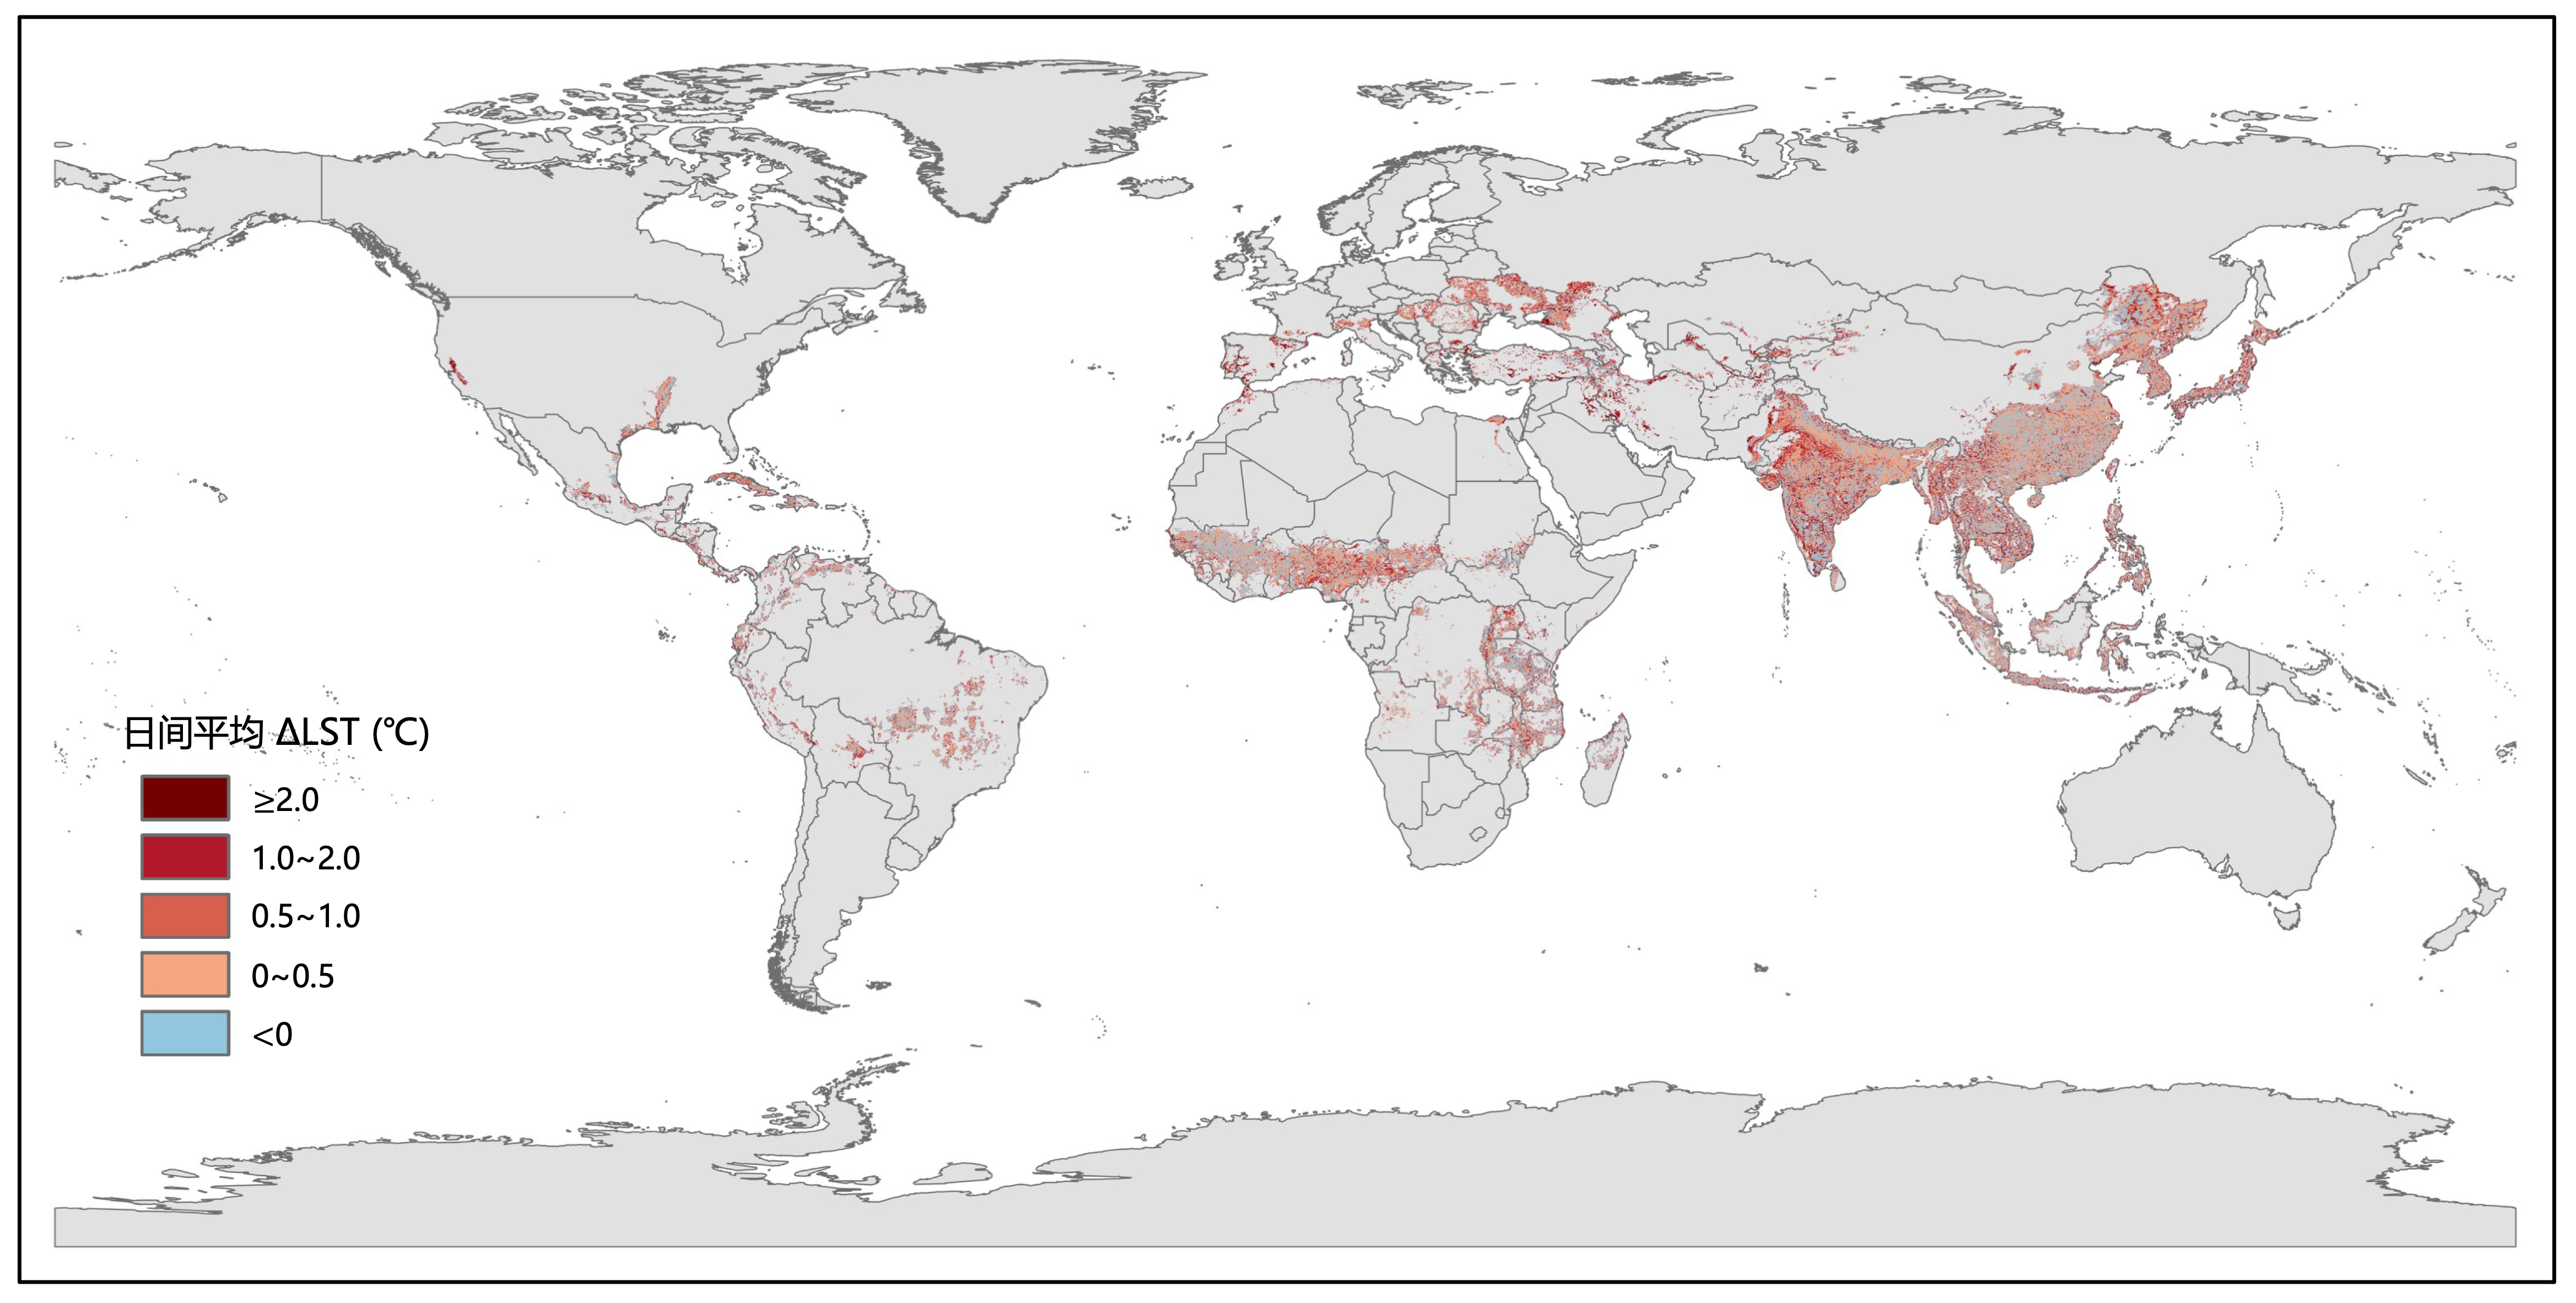
\includegraphics[width=0.99\linewidth]{figure/chapter4/mean_cooling_day.png}
    \bicaption[2003--2020 年全球水稻生长季日间 $\Delta \mathrm{LST}$ 多年平均值的空间分布]
    {2003--2020 年全球水稻生长季日间 $\Delta \mathrm{LST}$ 多年平均值的空间分布。$\Delta \mathrm{LST}$ 表示水稻生长季内周围非水稻耕地与水稻种植区之间的 LST 差值，正值表示水稻种植区相对于周边非水稻耕地更冷。}
    [Spatial distribution of the multiyear mean daytime $\Delta \mathrm{LST}$ during rice growing seasons worldwide, 2003–2020]
    {Spatial distribution of the multiyear mean daytime $\Delta \mathrm{LST}$ during rice growing seasons worldwide, 2003–2020. $\Delta \mathrm{LST}$ denotes the LST difference between surrounding non-paddy croplands and rice growing areas during rice growing seasons; positive values indicate cooler rice growing areas relative to surrounding non-paddy croplands.}
    \label{fig:global_daytime_dlst}
\end{figure}

% 空间分布
本节从空间分布和年际特征两个层面，分析全球水稻种植区生长季日间地表温度效应的总体表现。
2003—2020 年全球水稻生长季日间平均 $\Delta\mathrm{LST}$ 的空间分布表明，水稻种植区相对于周边非水稻耕地普遍表现出地表降温效应（图 \ref{fig:global_daytime_dlst}），说明该降温效应在全球主要水稻种植区具有较为广泛的空间分布。
同时，不同区域的降温幅度存在差异，表明水稻种植区地表降温效应具有空间异质性，可能受到局地水分背景、水稻种植区空间集聚程度以及周边非水稻耕地蒸散条件等因素的影响。
在水稻种植区集中度较高、灌溉水分输入较充分或周边非水稻耕地水分较为受限的地区，水稻种植区田面水蒸发和水稻冠层蒸腾所带来的潜热通量优势更容易转化为可观测的地表温度差异，从而表现出较强的相对降温。
在湿润背景较强、对照耕地同样具有较高蒸散发能力的区域，水稻种植区与非水稻耕地之间的温度差异则相对较弱；但也表现出稳定的正值 $\Delta \mathrm{LST}$，其幅度受到背景湿度、云雨条件、作物制度和非水稻耕地水分状态共同影响。
总体而言，全球主要水稻种植区普遍表现出日间相对降温，但降温幅度呈现明显的空间分异，可能与区域水热背景、水稻种植区空间分布特征及非水稻对照区域蒸散条件等因素有关。

% 年际稳定性
2003--2020 年间，全球水稻生长季日间平均 $\Delta \mathrm{LST}$ 始终保持为正值，年均值介于 0.2146--0.2699 $^{\circ}\mathrm{C}$ 之间（表 \ref{tab:global_daytime_delta_lst_uncertainty}）。
其中，2013 年均值最低，为 0.21 $^{\circ}\mathrm{C}$；2007 年均值最高，为 0.27 $^{\circ}\mathrm{C}$。
尽管不同年份之间存在一定波动，所有年份的日间平均 $\Delta \mathrm{LST}$ 均明显高于 0，说明水稻种植区相对于周边非水稻耕地的日间地表降温效应在整个研究期内持续存在。
从统计不确定性看，各年份均值标准误较小，约为 0.0057--0.0064 $^{\circ}\mathrm{C}$，95\% 置信区间均未跨越 0，说明全球平均日间降温信号具有较强的统计稳定性。
空间分布和年际变化结果共同说明，日间地表降温是全球水稻种植区中稳定存在的地表生物物理信号。

\begin{longtable}{@{}>{\centering\arraybackslash}p{0.12\textwidth}>{\centering\arraybackslash}p{0.14\textwidth}>{\centering\arraybackslash}p{0.18\textwidth}>{\centering\arraybackslash}p{0.18\textwidth}>{\centering\arraybackslash}p{0.18\textwidth}@{}}
    \bicaption{2003--2020 年全球水稻生长季日间平均 $\Delta \mathrm{LST}$ 及其不确定性估计}{Annual global mean daytime ΔLST and associated uncertainty during rice growing seasons, 2003–2020} 
    \label{tab:global_daytime_delta_lst_uncertainty} \\
    \toprule
    年份 & 均值 ($^{\circ}\mathrm{C}$) & 均值标准误 ($^{\circ}\mathrm{C}$) & 95\% 置信区间下限 ($^{\circ}\mathrm{C}$) & 95\% 置信区间上限 ($^{\circ}\mathrm{C}$) \\
    \midrule
    \endfirsthead
    \multicolumn{5}{c}{\zihao{5}\tablename\ \thetable{}\nobreakspace{}--\nobreakspace{}续表} \\
    \toprule
    年份 & 均值 ($^{\circ}\mathrm{C}$) & 均值标准误 ($^{\circ}\mathrm{C}$) & 95\% 置信区间下限 ($^{\circ}\mathrm{C}$) & 95\% 置信区间上限 ($^{\circ}\mathrm{C}$) \\
    \midrule
    \endhead
    \bottomrule
    \endfoot
    2003 & 0.2233 & 0.005774 & 0.2121 & 0.2348 \\
    2004 & 0.2498 & 0.006438 & 0.2372 & 0.2624 \\
    2005 & 0.2320 & 0.006214 & 0.2200 & 0.2444 \\
    2006 & 0.2326 & 0.005756 & 0.2216 & 0.2438 \\
    2007 & 0.2699 & 0.006332 & 0.2577 & 0.2822 \\
    2008 & 0.2336 & 0.005727 & 0.2225 & 0.2450 \\
    2009 & 0.2437 & 0.006050 & 0.2321 & 0.2557 \\
    2010 & 0.2288 & 0.005855 & 0.2172 & 0.2402 \\
    2011 & 0.2285 & 0.005929 & 0.2171 & 0.2404 \\
    2012 & 0.2451 & 0.006217 & 0.2330 & 0.2572 \\
    2013 & 0.2146 & 0.005712 & 0.2037 & 0.2260 \\
    2014 & 0.2379 & 0.006058 & 0.2263 & 0.2498 \\
    2015 & 0.2399 & 0.006035 & 0.2283 & 0.2517 \\
    2016 & 0.2339 & 0.005870 & 0.2226 & 0.2456 \\
    2017 & 0.2334 & 0.006113 & 0.2215 & 0.2455 \\
    2018 & 0.2561 & 0.006076 & 0.2443 & 0.2681 \\
    2019 & 0.2278 & 0.005988 & 0.2162 & 0.2396 \\
    2020 & 0.2336 & 0.005908 & 0.2224 & 0.2455 \\
\bottomrule
\end{longtable}

\subsection{全球夜间水稻种植区与非水稻种植区地表温差的空间分布与年际稳定性}
与日间相比，全球水稻生长季夜间 $\Delta \mathrm{LST}$ 的整体幅度明显减小。2003--2020 年多年平均的空间分布显示，全球大部分水稻种植区的夜间 $\Delta \mathrm{LST}$ 集中在 $-0.1$--$0.1~^{\circ}\mathrm{C}$ 范围内，局部地区呈现正值和负值相间分布，绝对值较大的区域相对有限（图 \ref{fig:global_nighttime_delta_lst}），表明水稻种植区与周边非水稻耕地之间的地表温度差异在夜间总体较弱。

\begin{figure}[htbp]
    \centering
    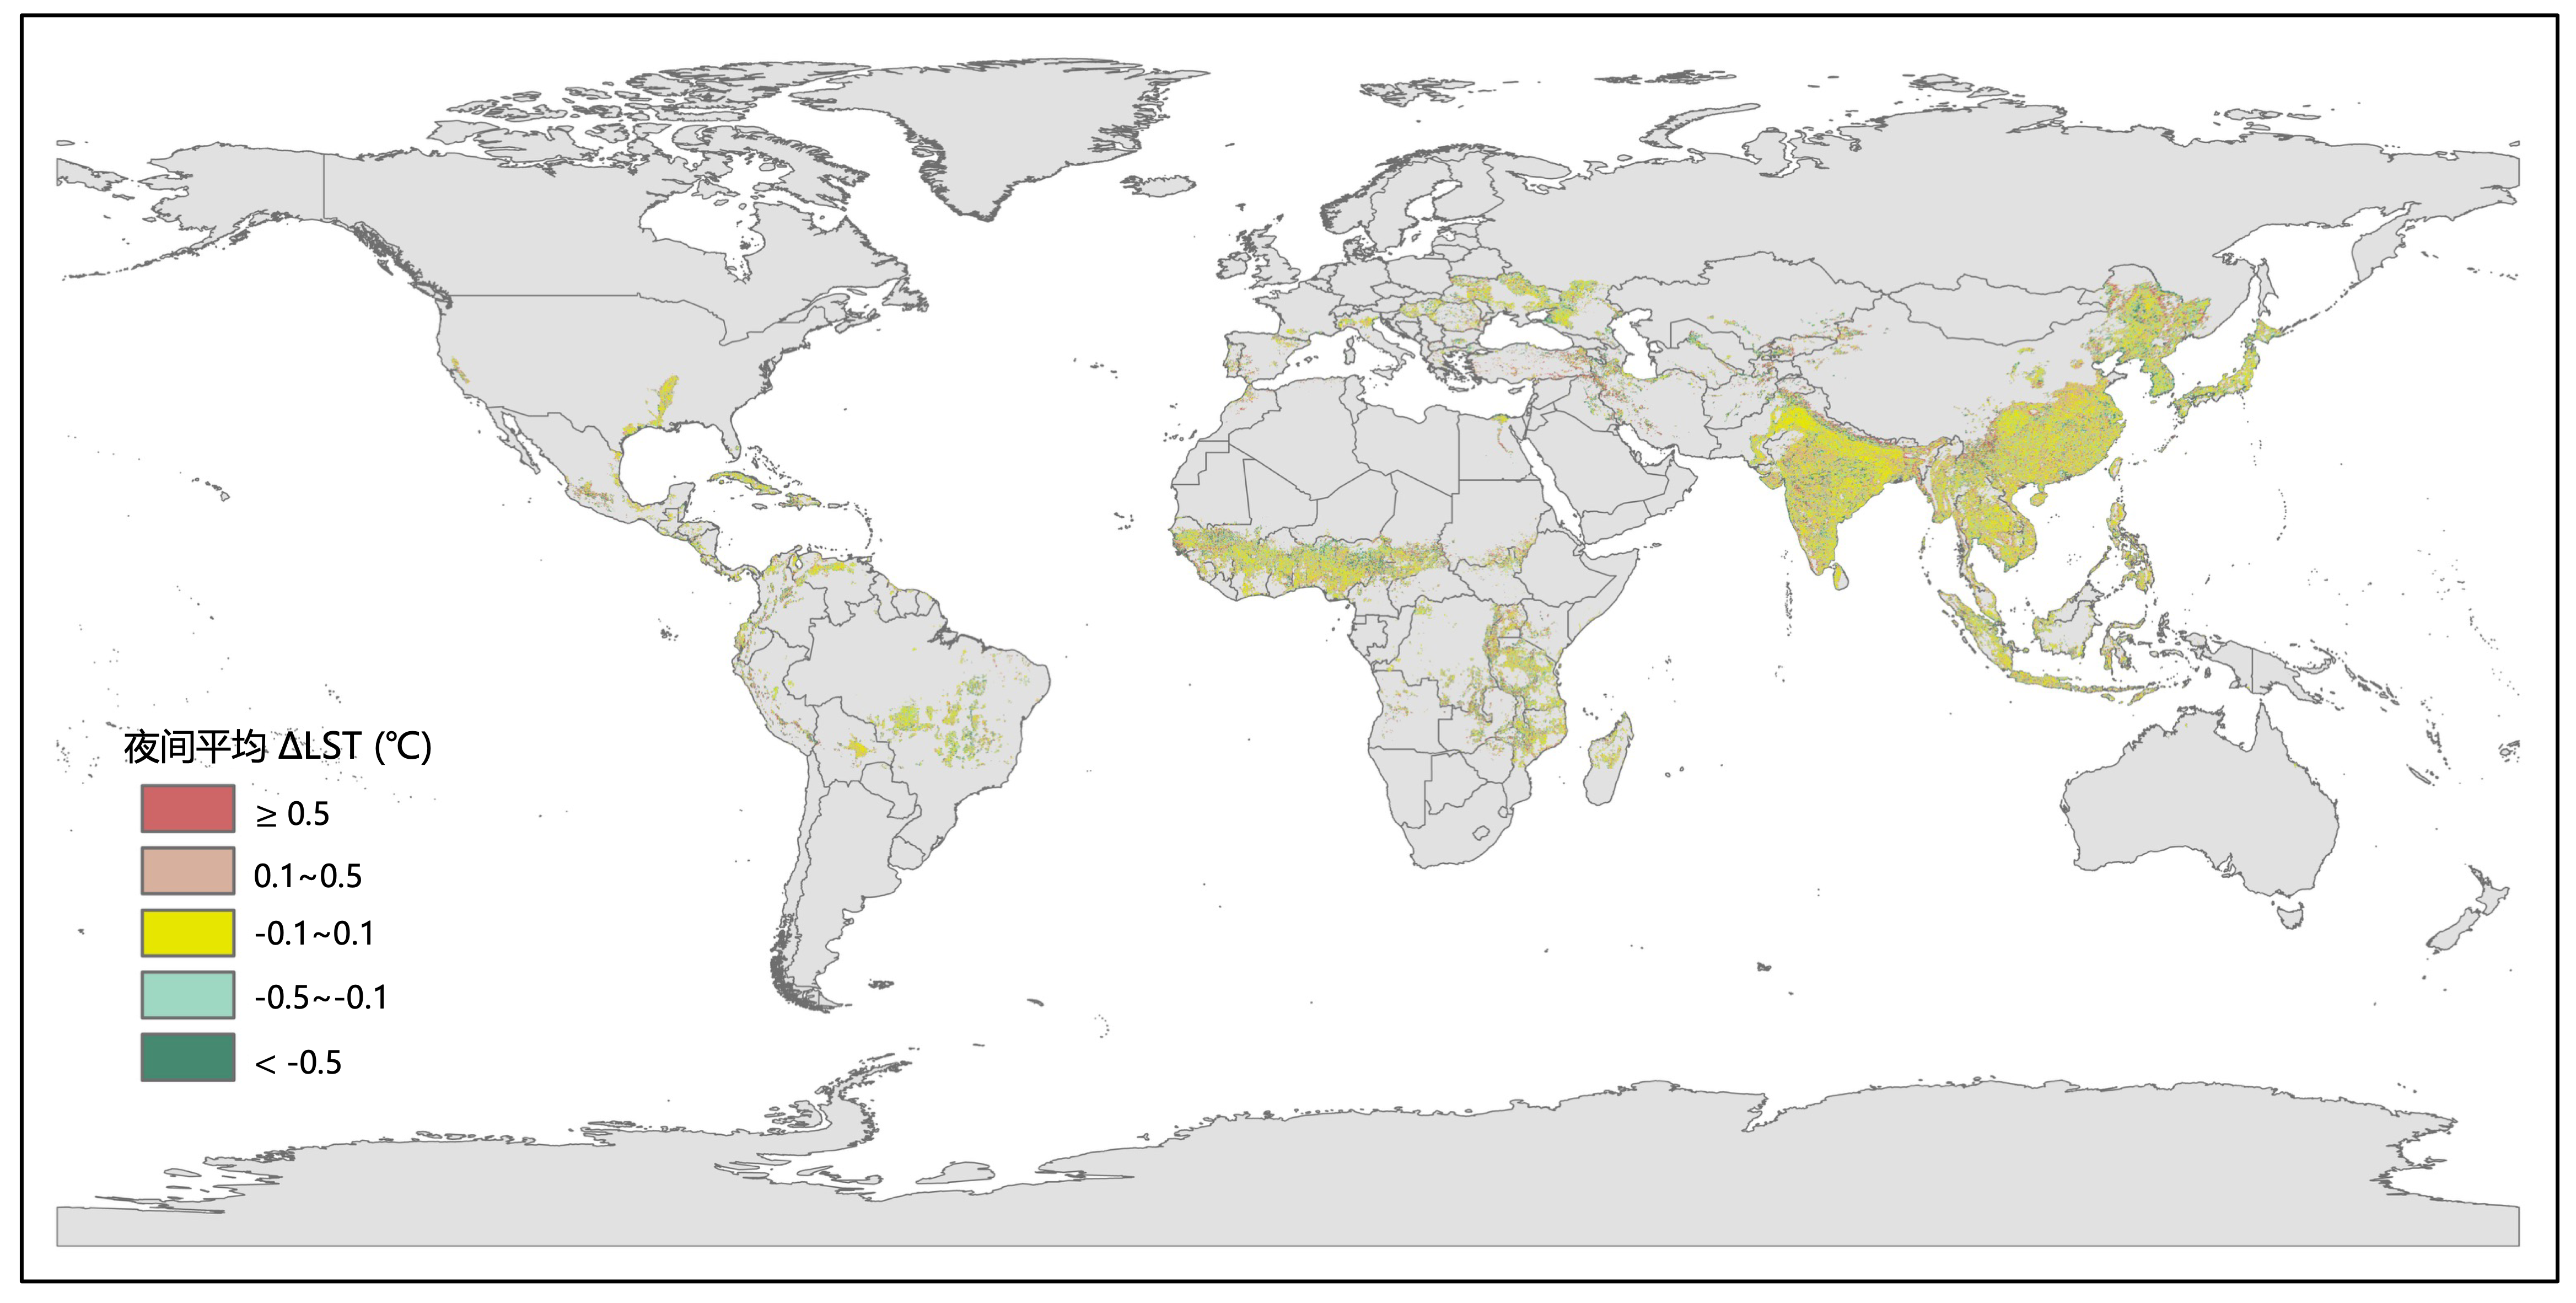
\includegraphics[width=0.95\linewidth]{figure/chapter4/mean_cooling_night.png}
    \bicaption[2003--2020 年全球水稻生长季夜间 $\Delta \mathrm{LST}$ 多年平均值的空间分布]
    {2003--2020 年全球水稻生长季夜间 $\Delta \mathrm{LST}$ 多年平均值的空间分布。$\Delta \mathrm{LST}$ 表示水稻生长季内周围非水稻耕地与水稻种植区之间的 LST 差值，正值表示水稻种植区相对于周边非水稻耕地更冷。}
    [Spatial distribution of the multiyear mean nighttime $\Delta \mathrm{LST}$ during rice growing seasons worldwide, 2003–2020]
    {Spatial distribution of the multiyear mean nighttime $\Delta \mathrm{LST}$ during rice growing seasons worldwide, 2003–2020. $\Delta \mathrm{LST}$ denotes the LST difference between surrounding non-paddy croplands and rice growing areas during rice growing seasons; positive values indicate cooler rice growing areas relative to surrounding non-paddy croplands.}
    \label{fig:global_nighttime_delta_lst}
\end{figure}

从年际特征看，2003--2020 年各年全球水稻生长季夜间平均 $\Delta \mathrm{LST}$ 均为微弱正值，介于 0.0077--0.0223~$^{\circ}\mathrm{C}$ 之间，各年度全球均值的多年平均约为 0.0135~$^{\circ}\mathrm{C}$（表 \ref{tab:global_nighttime_delta_lst_uncertainty}）。
各年均值标准误较为接近，且 95\% 置信区间均未跨越零，表明各年度均值估计的不确定性水平较为一致，夜间 $\Delta \mathrm{LST}$ 在年际间具有较好的统计稳健性。

总体而言，全球水稻种植区夜间 $\Delta \mathrm{LST}$ 在空间上普遍接近于零，在年际间保持相近数量级，表明日间较为明显的水稻种植区降温效应在夜间显著减弱。
这一昼夜差异可能与蒸散发的昼夜变化以及田面水和湿润土壤的热储特性有关 \cite{McDermid2023Irrigation,Xue2021RemoteSensing}。
日间短波辐射输入较强，在相近辐射背景下，水稻种植区较充足的水分供应使田面水蒸发、湿润土壤蒸发和水稻冠层蒸腾保持较高水平，促使更多可用能量分配至潜热通量，从而削弱显热加热和地表升温。同时，田面水和湿润土壤较高的有效热惯量能够减缓日间地表温度上升，进一步强化水稻种植区相对于非水稻耕地的日间低温特征。
夜间短波辐射输入停止，蒸发和植被蒸腾明显减弱，由水分供应差异引起的潜热通量差异随之缩小。与此同时，田面水和湿润土壤在日间储存的热量于夜间逐渐释放，可能使水稻种植区的冷却速率相对减缓，从而部分抵消日间形成的低温差异\cite{Liu2022AgForMet,Xue2021RemoteSensing}。上述过程共同促使水稻种植区与非水稻耕地之间的夜间地表温度差异收敛，使夜间 $\Delta \mathrm{LST}$ 总体接近零。

\begin{longtable}{@{}>{\centering\arraybackslash}p{0.12\textwidth}>{\centering\arraybackslash}p{0.14\textwidth}>{\centering\arraybackslash}p{0.18\textwidth}>{\centering\arraybackslash}p{0.18\textwidth}>{\centering\arraybackslash}p{0.18\textwidth}@{}}
    \bicaption{2003--2020 年全球水稻生长季夜间平均 $\Delta \mathrm{LST}$ 及其不确定性估计}{Annual global mean nighttime ΔLST and associated uncertainty during rice growing seasons, 2003–2020} \label{tab:global_nighttime_delta_lst_uncertainty} \\
    \toprule
    年份 & 均值 ($^{\circ}\mathrm{C}$) & 均值标准误 ($^{\circ}\mathrm{C}$) & 95\% 置信区间下限 ($^{\circ}\mathrm{C}$) & 95\% 置信区间上限 ($^{\circ}\mathrm{C}$) \\
    \midrule
    \endfirsthead
    \multicolumn{5}{c}{\zihao{5}\tablename\ \thetable{}\nobreakspace{}--\nobreakspace{}续表} \\
    \toprule
    年份 & 均值 ($^{\circ}\mathrm{C}$) & 均值标准误 ($^{\circ}\mathrm{C}$) & 95\% 置信区间下限 ($^{\circ}\mathrm{C}$) & 95\% 置信区间上限 ($^{\circ}\mathrm{C}$) \\
    \midrule
    \endhead
    \bottomrule
    \endfoot
2003 & 0.007687 & 0.001875 & 0.003956 & 0.01136 \\
2004 & 0.008449 & 0.002065 & 0.004474 & 0.01253 \\
2005 & 0.01808 & 0.001732 & 0.01470 & 0.02150 \\
2006 & 0.01311 & 0.001741 & 0.009729 & 0.01658 \\
2007 & 0.01298 & 0.002028 & 0.009019 & 0.01695 \\
2008 & 0.01819 & 0.001794 & 0.01457 & 0.02170 \\
2009 & 0.01251 & 0.001740 & 0.009115 & 0.01595 \\
2010 & 0.01664 & 0.001902 & 0.01292 & 0.02042 \\
2011 & 0.009387 & 0.001801 & 0.005846 & 0.01282 \\
2012 & 0.01318 & 0.001876 & 0.009485 & 0.01685 \\
2013 & 0.01103 & 0.001769 & 0.007612 & 0.01452 \\
2014 & 0.01390 & 0.001698 & 0.01057 & 0.01727 \\
2015 & 0.01575 & 0.001837 & 0.01208 & 0.01932 \\
2016 & 0.01306 & 0.001773 & 0.009581 & 0.01658 \\
2017 & 0.01167 & 0.001944 & 0.007949 & 0.01553 \\
2018 & 0.01073 & 0.001756 & 0.007292 & 0.01415 \\
2019 & 0.01405 & 0.001813 & 0.01050 & 0.01764 \\
2020 & 0.02231 & 0.001862 & 0.01863 & 0.02598 \\
\bottomrule
\end{longtable}

\clearpage

\subsection{不同气候区水稻种植区与非水稻种植区的地表温差评估}
卫星 LST 观测条件、背景耕地水分状态、蒸散需求及水稻生长过程均可能随气候背景而变化，从而使水稻种植区与非水稻耕地之间的地表温度差异呈现区域分异。
为比较不同气候背景下水稻种植区 $\Delta \mathrm{LST}$ 的方向和强度，本研究依据柯本--盖格气候分类（Köppen--Geiger climate classification）的一级气候类型进行分区统计，包括赤道气候（A）、干旱气候（B）、暖温带气候（C）和雪气候（D）四类（图~\ref{fig:main_climate_zones}）。极地气候（E）因水稻种植区分布极少，未纳入分析。
各气候区分别统计日间和夜间 $\Delta \mathrm{LST}$ 的均值、均值标准误和 95\% 置信区间，以表征分区估计结果及其不确定性。

\begin{figure}[htbp]
    \centering
    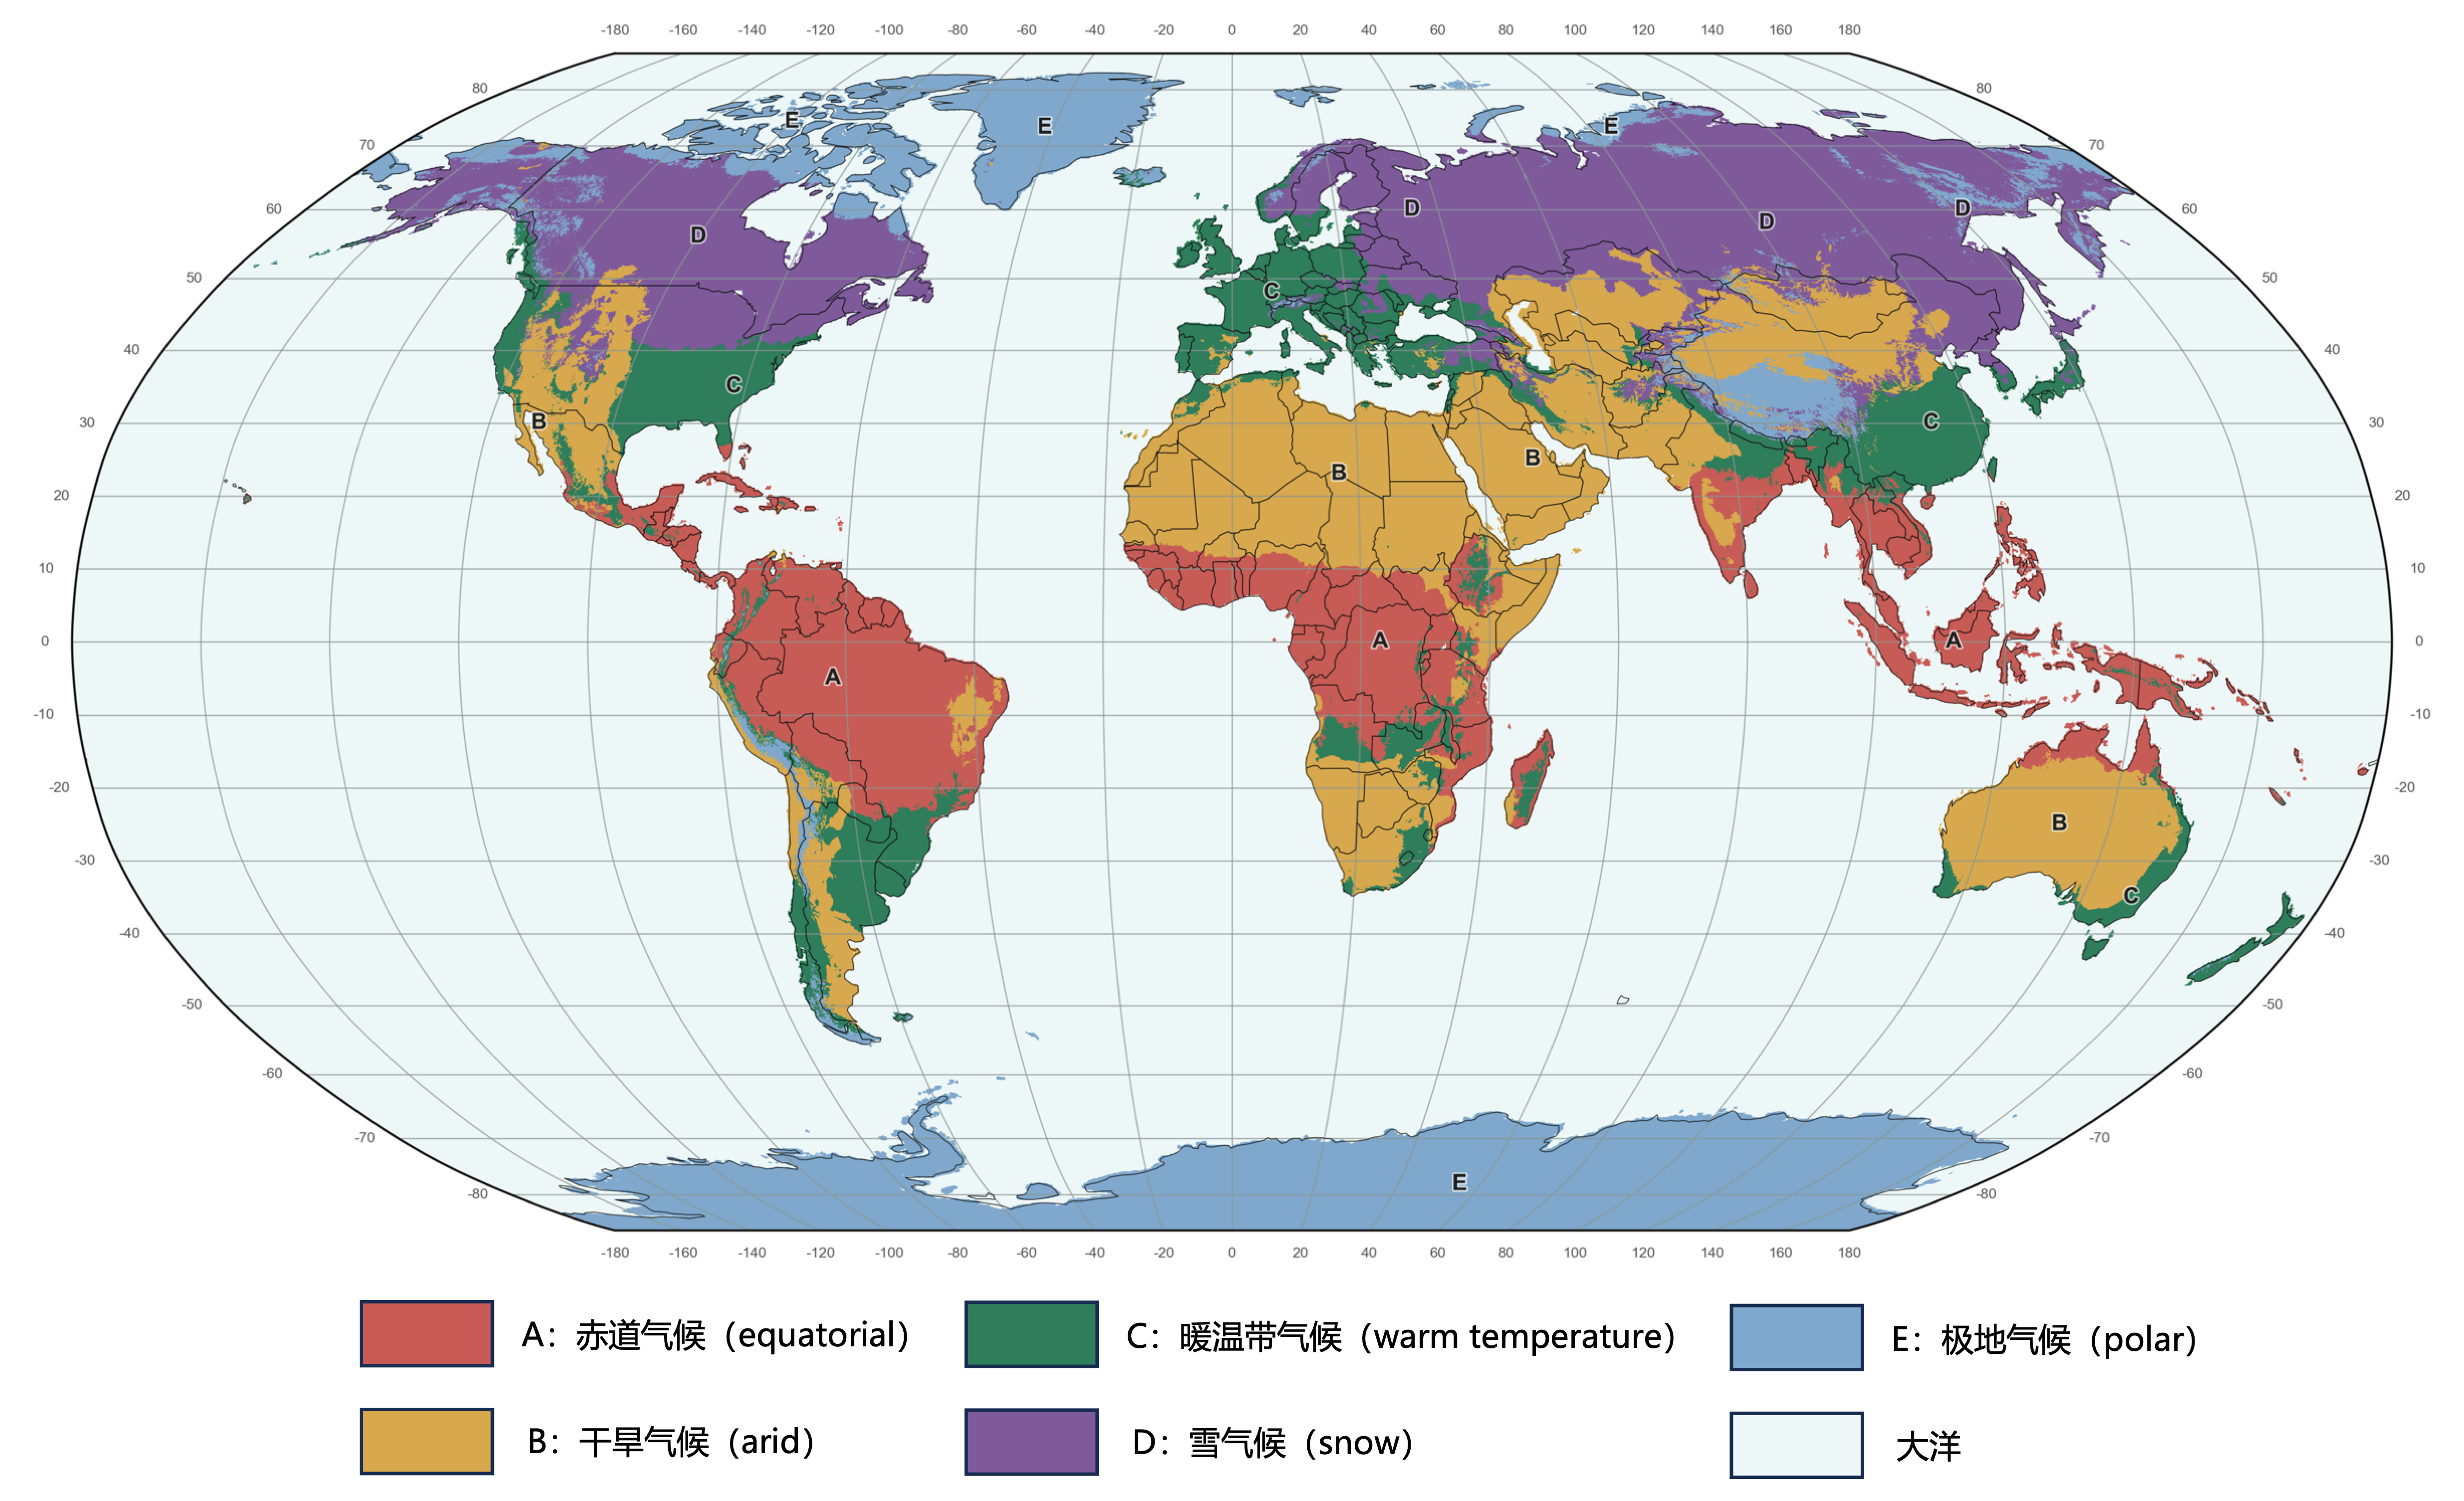
\includegraphics[width=0.95\linewidth]{figure/chapter4/main_climate_zones_2017.png}
    \bicaption[全球柯本—盖格一级气候类型的空间分布]{全球柯本—盖格一级气候类型的空间分布。一级气候类型（main climates，以分类编码首字母区分）包括赤道气候（A）、干旱气候（B）、暖温带气候（C）、雪气候（D）和极地气候（E）五大类。制图数据为柯本--盖格气候分类 2017 年 3 月更新版本，来自 \url{https://koeppen-geiger.vu-wien.ac.at/}，获取于 2025 年 9 月 6 日。}[Köppen--Geiger main climates]{Köppen--Geiger main climates (first-level classification denoted by the first letter of the climate code): equatorial (A), arid (B), warm temperate (C), snow (D), and polar (E). The map is based on the March 2017 version of the Köppen--Geiger climate classification, downloaded from \url{https://koeppen-geiger.vu-wien.ac.at/}, accessed on September 6, 2025.}
    \label{fig:main_climate_zones}
\end{figure}

% 日间结果
分区统计结果表明，四个主要气候区的日间平均 $\Delta \mathrm{LST}$ 均为正值（表 \ref{tab:climate_day_dlst_uncertainty}）。
其中，干旱气候区的日间平均 $\Delta \mathrm{LST}$ 最高，为 0.4729~$^{\circ}\mathrm{C}$；雪气候区次之（0.2592~$^{\circ}\mathrm{C}$）；暖温带气候区和赤道气候区分别为 0.1372~$^{\circ}\mathrm{C}$ 和 0.1260~$^{\circ}\mathrm{C}$。
各气候区日间平均 $\Delta \mathrm{LST}$ 的 95\% 置信区间均未跨越零，表明水稻种植区在不同气候区均表现出相对于周边非水稻耕地的日间降温特征。

% \begin{table}[htbp]
%     \centering
%     \bicaption{不同 Köppen--Geiger 气候区内 $\Delta \mathrm{LST}$ 的不确定性估计}{Uncertainty of $\Delta \mathrm{LST}$ across Köppen--Geiger climate zones} \label{tab:climate_zone_delta_lst_uncertainty}
%     \small
%     \setlength{\tabcolsep}{3pt}
%     \begin{tabular}{@{}>{\centering\arraybackslash}p{0.06\textwidth}>{\raggedright\arraybackslash}p{0.12\textwidth}>{\centering\arraybackslash}p{0.07\textwidth}>{\centering\arraybackslash}p{0.07\textwidth}>{\centering\arraybackslash}p{0.07\textwidth}>{\centering\arraybackslash}p{0.08\textwidth}>{\centering\arraybackslash}p{0.09\textwidth}>{\centering\arraybackslash}p{0.09\textwidth}>{\centering\arraybackslash}p{0.09\textwidth}@{}}
%         \toprule
%         时段 & 气候区 & \multicolumn{3}{c}{LST 均方根误差 ($^{\circ}\mathrm{C}$)} & $\Delta \mathrm{LST}$ 均值 ($^{\circ}\mathrm{C}$) & 均值标准误 ($^{\circ}\mathrm{C}$) & 95\% 置信区间下限 ($^{\circ}\mathrm{C}$) & 95\% 置信区间上限 ($^{\circ}\mathrm{C}$) \\
%         \cmidrule(lr){3-5}
%         & & 25\% 排除 & 50\% 排除 & 75\% 排除 & & & & \\
%         \midrule
%         日间 & 赤道气候区 & 1.97 & 1.96 & 2.03 & 0.1260 & 0.003566 & 0.1190 & 0.1330 \\
%         日间 & 干旱气候区 & 1.40 & 1.42 & 1.64 & 0.4729 & 0.01196 & 0.4497 & 0.4962 \\
%         日间 & 暖温带气候区 & 1.81 & 1.79 & 2.05 & 0.1372 & 0.003946 & 0.1296 & 0.1450 \\
%         日间 & 雪气候区 & 2.17 & 2.25 & 2.50 & 0.2592 & 0.01114 & 0.2380 & 0.2817 \\
%         夜间 & 赤道气候区 & 1.24 & 1.21 & 1.33 & 0.01110 & 0.001400 & 0.008387 & 0.01386 \\
%         夜间 & 干旱气候区 & 1.03 & 1.19 & 1.30 & 0.01939 & 0.002917 & 0.01365 & 0.02520 \\
%         夜间 & 暖温带气候区 & 1.11 & 1.23 & 1.40 & 0.01773 & 0.001471 & 0.01485 & 0.02058 \\
%         夜间 & 雪气候区 & 1.80 & 1.81 & 1.97 & -0.02839 & 0.005069 & -0.03829 & -0.01855 \\
%         \bottomrule
%     \end{tabular}
% \end{table}

\begin{table}[htbp]
    \centering
    \bicaption{不同柯本--盖格气候区日间平均 $\Delta \mathrm{LST}$ 的不确定性估计}
    {Uncertainty of mean daytime $\Delta \mathrm{LST}$ across Köppen--Geiger climate zones}
    \label{tab:climate_day_dlst_uncertainty}
    % \small
    \setlength{\tabcolsep}{6pt}
    \begin{tabular}{@{}>{\raggedright\arraybackslash}p{0.16\textwidth}
                    >{\centering\arraybackslash}p{0.14\textwidth}
                    >{\centering\arraybackslash}p{0.14\textwidth}
                    >{\centering\arraybackslash}p{0.18\textwidth}
                    >{\centering\arraybackslash}p{0.18\textwidth}@{}}
        \toprule
        气候区
        & $\Delta \mathrm{LST}$ 均值 ($^{\circ}\mathrm{C}$) 
        & 均值标准误 ($^{\circ}\mathrm{C}$) 
        & 95\% 置信区间下限 ($^{\circ}\mathrm{C}$) 
        & 95\% 置信区间上限 ($^{\circ}\mathrm{C}$) \\
        \midrule
        赤道气候 & 0.1260 & 0.003566 & 0.1190 & 0.1330 \\
        干旱气候 & 0.4729 & 0.01196  & 0.4497 & 0.4962 \\
        暖温带气候 & 0.1372 & 0.003946 & 0.1296 & 0.1450 \\
        雪气候 & 0.2592 & 0.01114  & 0.2380 & 0.2817 \\
        \bottomrule
    \end{tabular}
\end{table}

不同气候区的日间 $\Delta \mathrm{LST}$ 差异表明，水稻种植区的地表降温不仅取决于稻田自身的水分供应和蒸散过程，还受到区域背景水分状况与能量条件的共同调节。
干旱气候区较高的日间 $\Delta \mathrm{LST}$ 可能与水稻种植区和非水稻耕地之间较大的水分条件差异有关。在背景非水稻耕地蒸散受到较强水分限制的情况下，水稻种植区较充足的水分供应可能增强两类耕地之间的蒸散和地表能量分配差异，水稻种植区潜热通量优势更加突出，从而形成更明显的地表温度差异 \cite{Seneviratne2010SoilMoisture,McDermid2023Irrigation}。
在赤道和暖温带气候区，背景水分条件相对充足，非水稻耕地同样可能具有较高的蒸散能力，水稻种植区与对照耕地之间的热状态差异相对较小。
雪气候区较大的日间 $\Delta \mathrm{LST}$ 可能与其水稻生长季集中于暖季有关。暖季通常具有较强的日间辐射和较高的潜在蒸散需求，有利于水稻种植区与非水稻耕地之间形成较明显的能量分配差异。不过，该结果也可能受到非水稻耕地水分状况、水稻种植区空间集聚程度以及区域样本构成的共同影响，具体机制仍需结合辐射、土壤水分和蒸散发数据进一步检验。

% 夜间结果
夜间 $\Delta \mathrm{LST}$ 与日间明显不同（表 \ref{tab:climate_night_dlst_uncertainty}）。
赤道气候区、干旱气候区和暖温带气候区的夜间平均 $\Delta \mathrm{LST}$ 分别为 0.01110、0.01939 和 0.01773~$^{\circ}\mathrm{C}$，均为接近零的弱正值；
雪气候区夜间平均 $\Delta \mathrm{LST}$ 为 $-0.02839~^{\circ}\mathrm{C}$，表明该气候区水稻种植区的夜间地表温度略高于周边非水稻耕地。
各气候区夜间平均 $\Delta \mathrm{LST}$ 的 95\% 置信区间均较窄且均值标准误较小，说明各分区夜间 $\Delta \mathrm{LST}$ 均值估计具有统计稳健性。
夜间 $\Delta \mathrm{LST}$ 的绝对量级均远低于日间，表明各气候区水稻种植区与非水稻耕地之间的夜间地表温度差异普遍较小。

\begin{table}[htbp]
    \centering
    \bicaption{不同柯本--盖格气候区夜间平均 $\Delta \mathrm{LST}$ 的不确定性估计}
    {Uncertainty of mean nighttime $\Delta \mathrm{LST}$ across Köppen--Geiger climate zones}
    \label{tab:climate_night_dlst_uncertainty}
    % \small
    \setlength{\tabcolsep}{6pt}
    \begin{tabular}{@{}>{\raggedright\arraybackslash}p{0.16\textwidth}
                    >{\centering\arraybackslash}p{0.14\textwidth}
                    >{\centering\arraybackslash}p{0.14\textwidth}
                    >{\centering\arraybackslash}p{0.18\textwidth}
                    >{\centering\arraybackslash}p{0.18\textwidth}@{}}
        \toprule
        气候区
        & $\Delta \mathrm{LST}$ 均值 ($^{\circ}\mathrm{C}$) 
        & 均值标准误 ($^{\circ}\mathrm{C}$) 
        & 95\% 置信区间下限 ($^{\circ}\mathrm{C}$) 
        & 95\% 置信区间上限 ($^{\circ}\mathrm{C}$) \\
        \midrule
        赤道气候 & 0.01110  & 0.001400 & 0.008387 & 0.01386 \\
        干旱气候 & 0.01939  & 0.002917 & 0.01365  & 0.02520 \\
        暖温带气候 & 0.01773  & 0.001471 & 0.01485  & 0.02058 \\
        雪气候 & -0.02839 & 0.005069 & -0.03829 & -0.01855 \\
        \bottomrule
    \end{tabular}
\end{table}

综合来看，水稻种植区相对于非水稻耕地的日间地表降温在四个主要气候区均表现为正值，但降温强度具有明显的气候区差异。相比之下，各气候区夜间 $\Delta \mathrm{LST}$ 均接近零，说明水稻种植区地表温度效应具有昼夜差异。

\section{水稻种植区降温效应随十公里网格内水稻种植区比例的变化}
\label{sec:paddy_proportion}

本节分析十公里网格内水稻种植区比例（Paddy Proportion）对日间 $\Delta \mathrm{LST}$ 的影响，以考察水稻种植区降温效应与局地水稻种植区面积占比之间的关系。
% 十公里网格内水稻种植区比例表示局地景观中水稻种植区所占的面积份额，用于表征局地景观中水稻种植区覆盖程度。
本研究在 MODIS 500 m 栅格基础上构建由 $20\times20$ 个像元组成的规则统计网格，每个网格约对应 $10~\mathrm{km}\times10~\mathrm{km}$ 的空间范围（图 \ref{fig:NPL_definition_a}）。
十公里网格内水稻种植区比例定义为：
\begin{equation}
    P_{\mathrm{paddy}}=
    \frac{N_{\mathrm{paddy}}}{20\times20},
\end{equation}
其中，$N_{\mathrm{paddy}}$ 为网格内水稻种植区像元数，$P_{\mathrm{paddy}}$ 取值范围为 0--1；换算为百分比时为 $100P_{\mathrm{paddy}}\%$。
% \begin{equation}
%     P_{\mathrm{paddy}}=\frac{N_{\mathrm{paddy}}}{20\times20}\times100\%,
% \end{equation}
% 其中，$N_{\mathrm{paddy}}$ 为网格内水稻种植区像元数，$P_{\mathrm{paddy}}$ 以百分数表示。
随后，本研究采用等宽分箱（equal-width binning）方法，以 0.01（即 1 个百分点）为箱宽，对十公里网格内水稻种植区比例进行划分。第 $k$ 组对应的十公里网格内水稻种植区比例范围为 $((k-1)/100,k/100]$，即十公里网格内水稻种植区比例大于 $(k-1)\%$ 且不高于 $k\%$。%（$(k-1\%,k\%]$）。
将各网格对应的 $\Delta \mathrm{LST}$ 样本归入相应比例组，并统计各组在 2003--2020 年期间的多年平均值及其均值标准误。
为减小网格内水稻样本数量过少对统计结果稳定性的影响，本文仅保留 $P_{\mathrm{paddy}}\geq0.20$ 的网格，即每个网格至少包含 80 个水稻像元。
%该阈值作为样本筛选条件，仅用于保证网格内具有一定数量的水稻样本，不代表水稻种植区降温效应存在普适的比例临界值。%该阈值属于样本质量控制条件，不表示水稻种植区降温效应存在普适的比例临界点。

\begin{figure}[htbp]
    \centering
    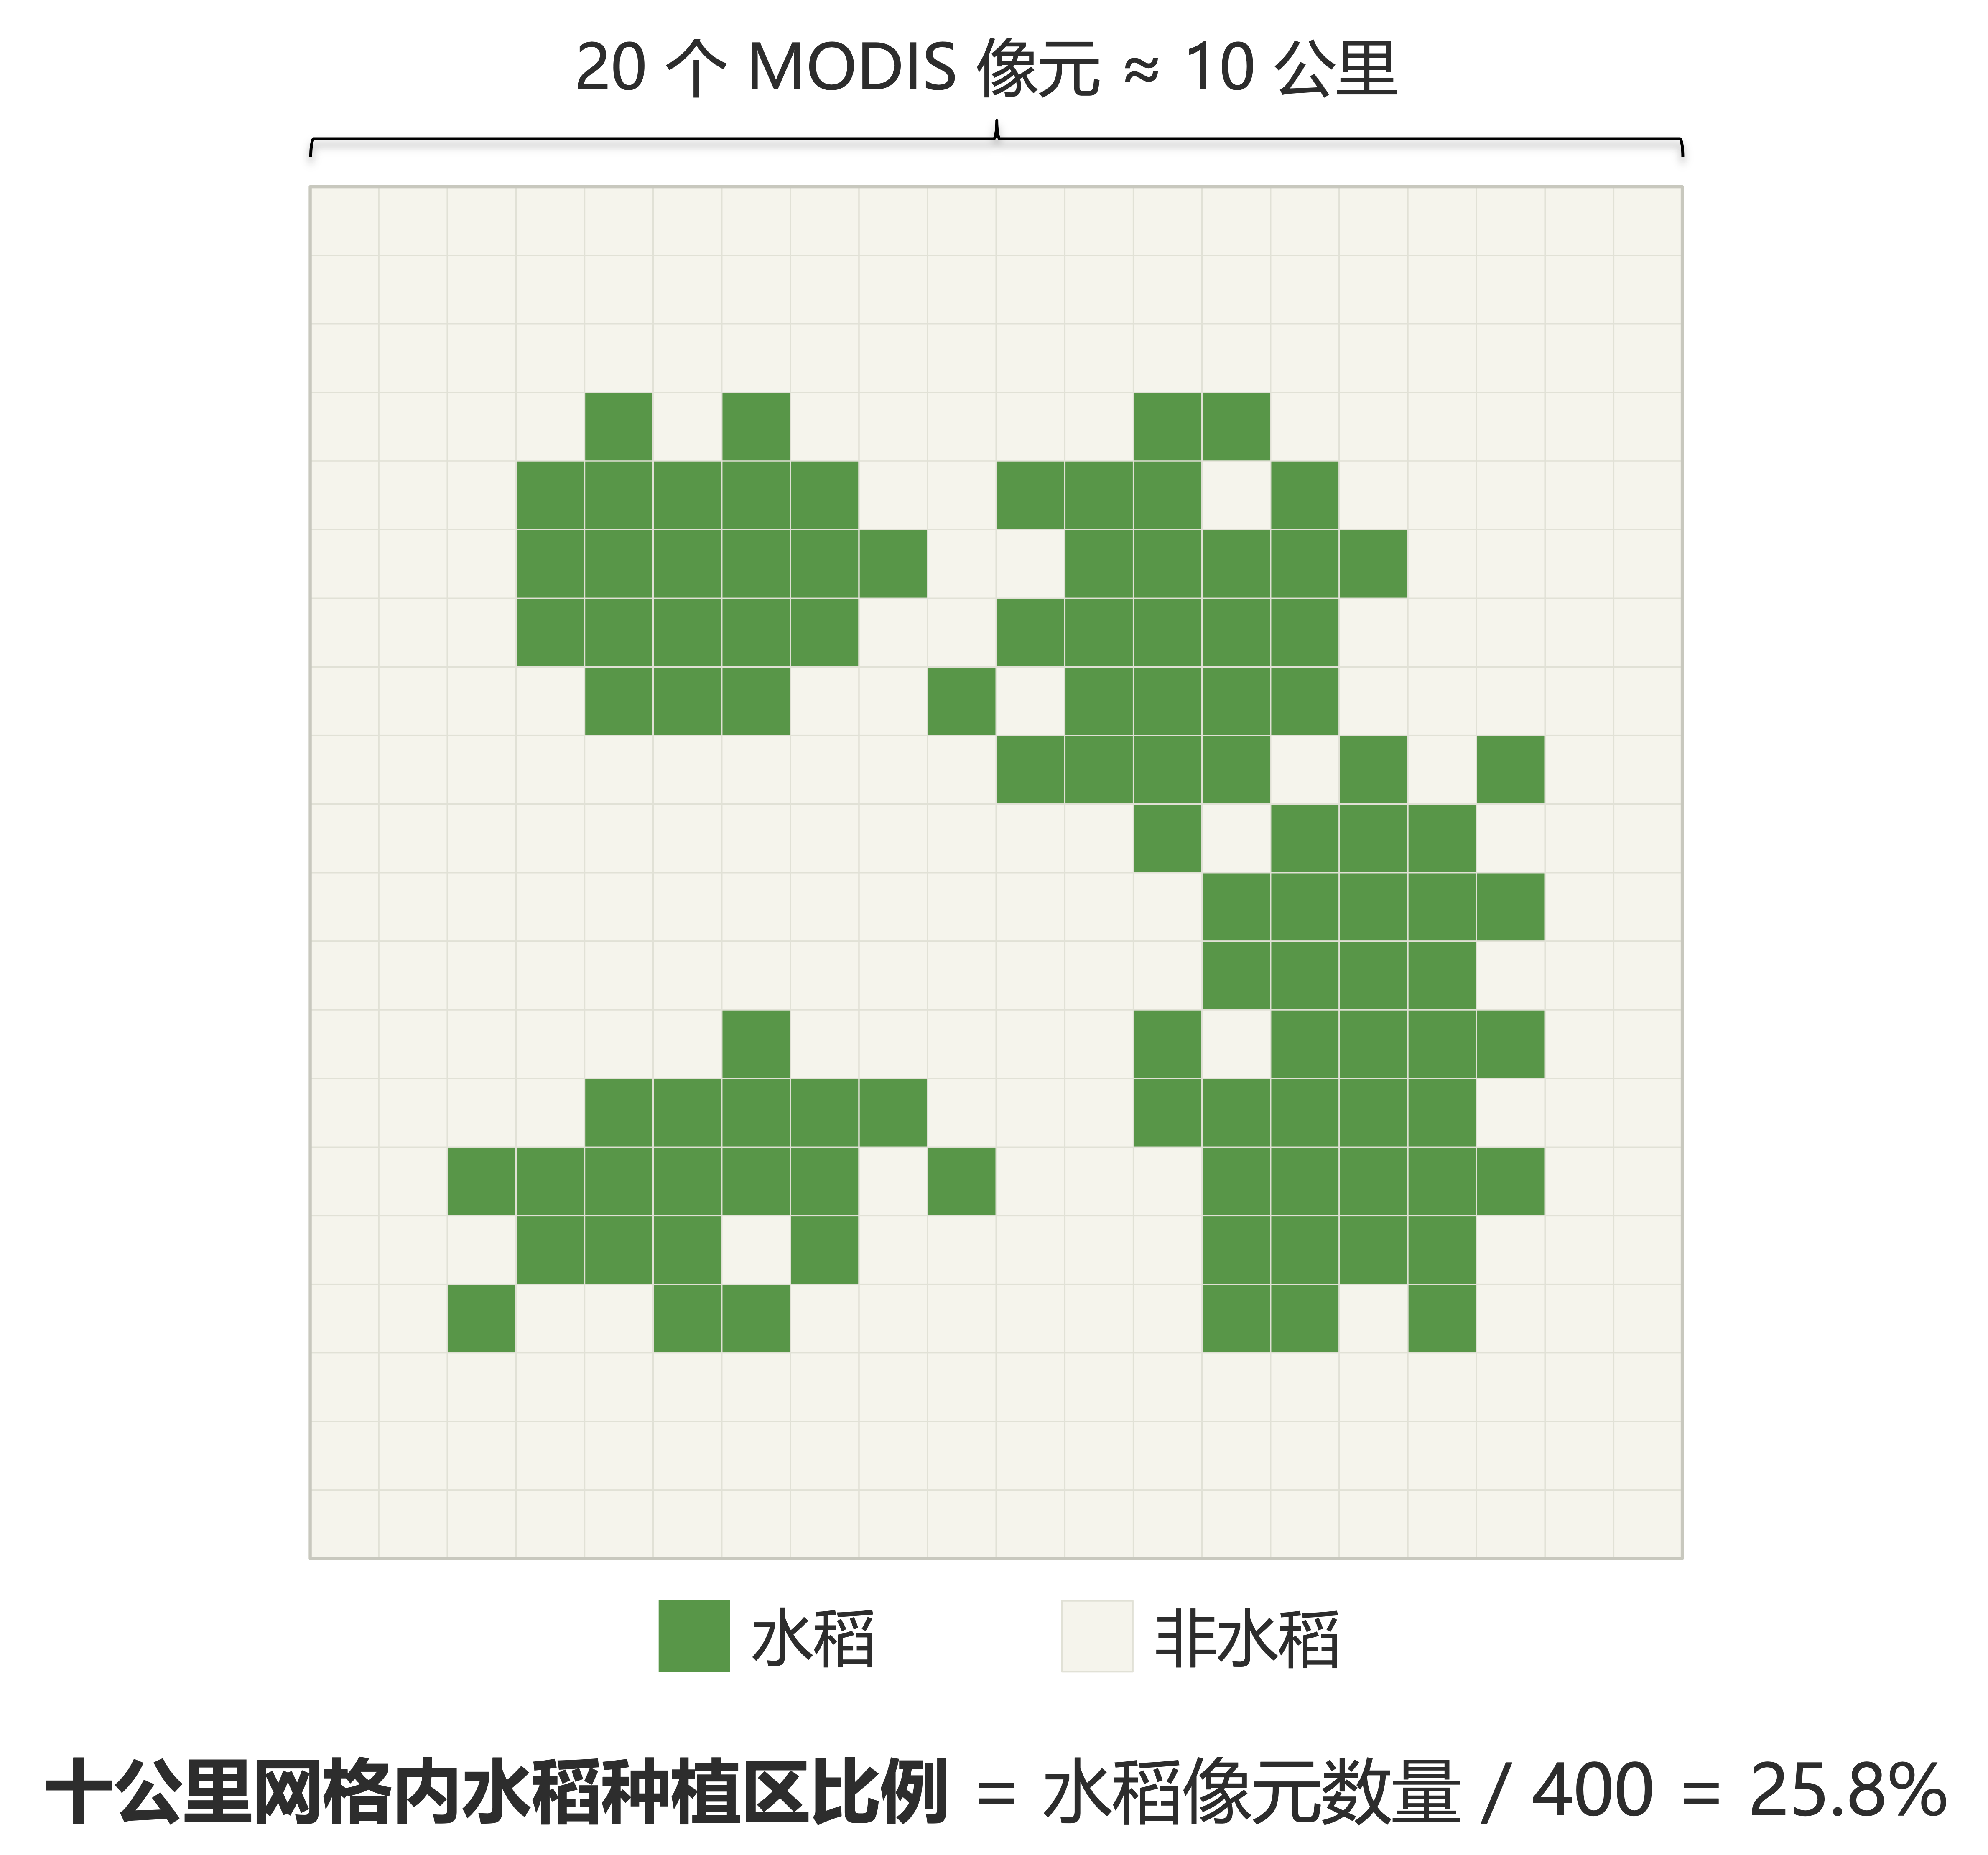
\includegraphics[width=0.5\linewidth]{figure/chapter4/NPL_definition_a.png}
    \bicaption[十公里网格内水稻种植区比例示意图]
    {十公里网格内水稻种植区比例示意图。
    十公里网格内水稻种植区比例表示 $20 \times 20$ 个 MODIS 500 m 像元
    （约 $10~\mathrm{km} \times 10~\mathrm{km}$）内水稻种植区像元数占总像元数的百分比。
    %绿色表示水稻种植区像元，浅米色表示非水稻农田。
    }
    [Schematic illustration of Paddy Proportion]
    {Schematic illustration of Paddy Proportion.
    Paddy Proportion is calculated as the percentage of paddy rice pixels within a $20 \times 20$ MODIS 500 m grid, approximately $10~\mathrm{km} \times 10~\mathrm{km}$.
    %Green denotes paddy rice pixels, and light beige denotes non-paddy cropland.
    }
    \label{fig:NPL_definition_a}
\end{figure}

\begin{figure}[htbp]
    \centering
    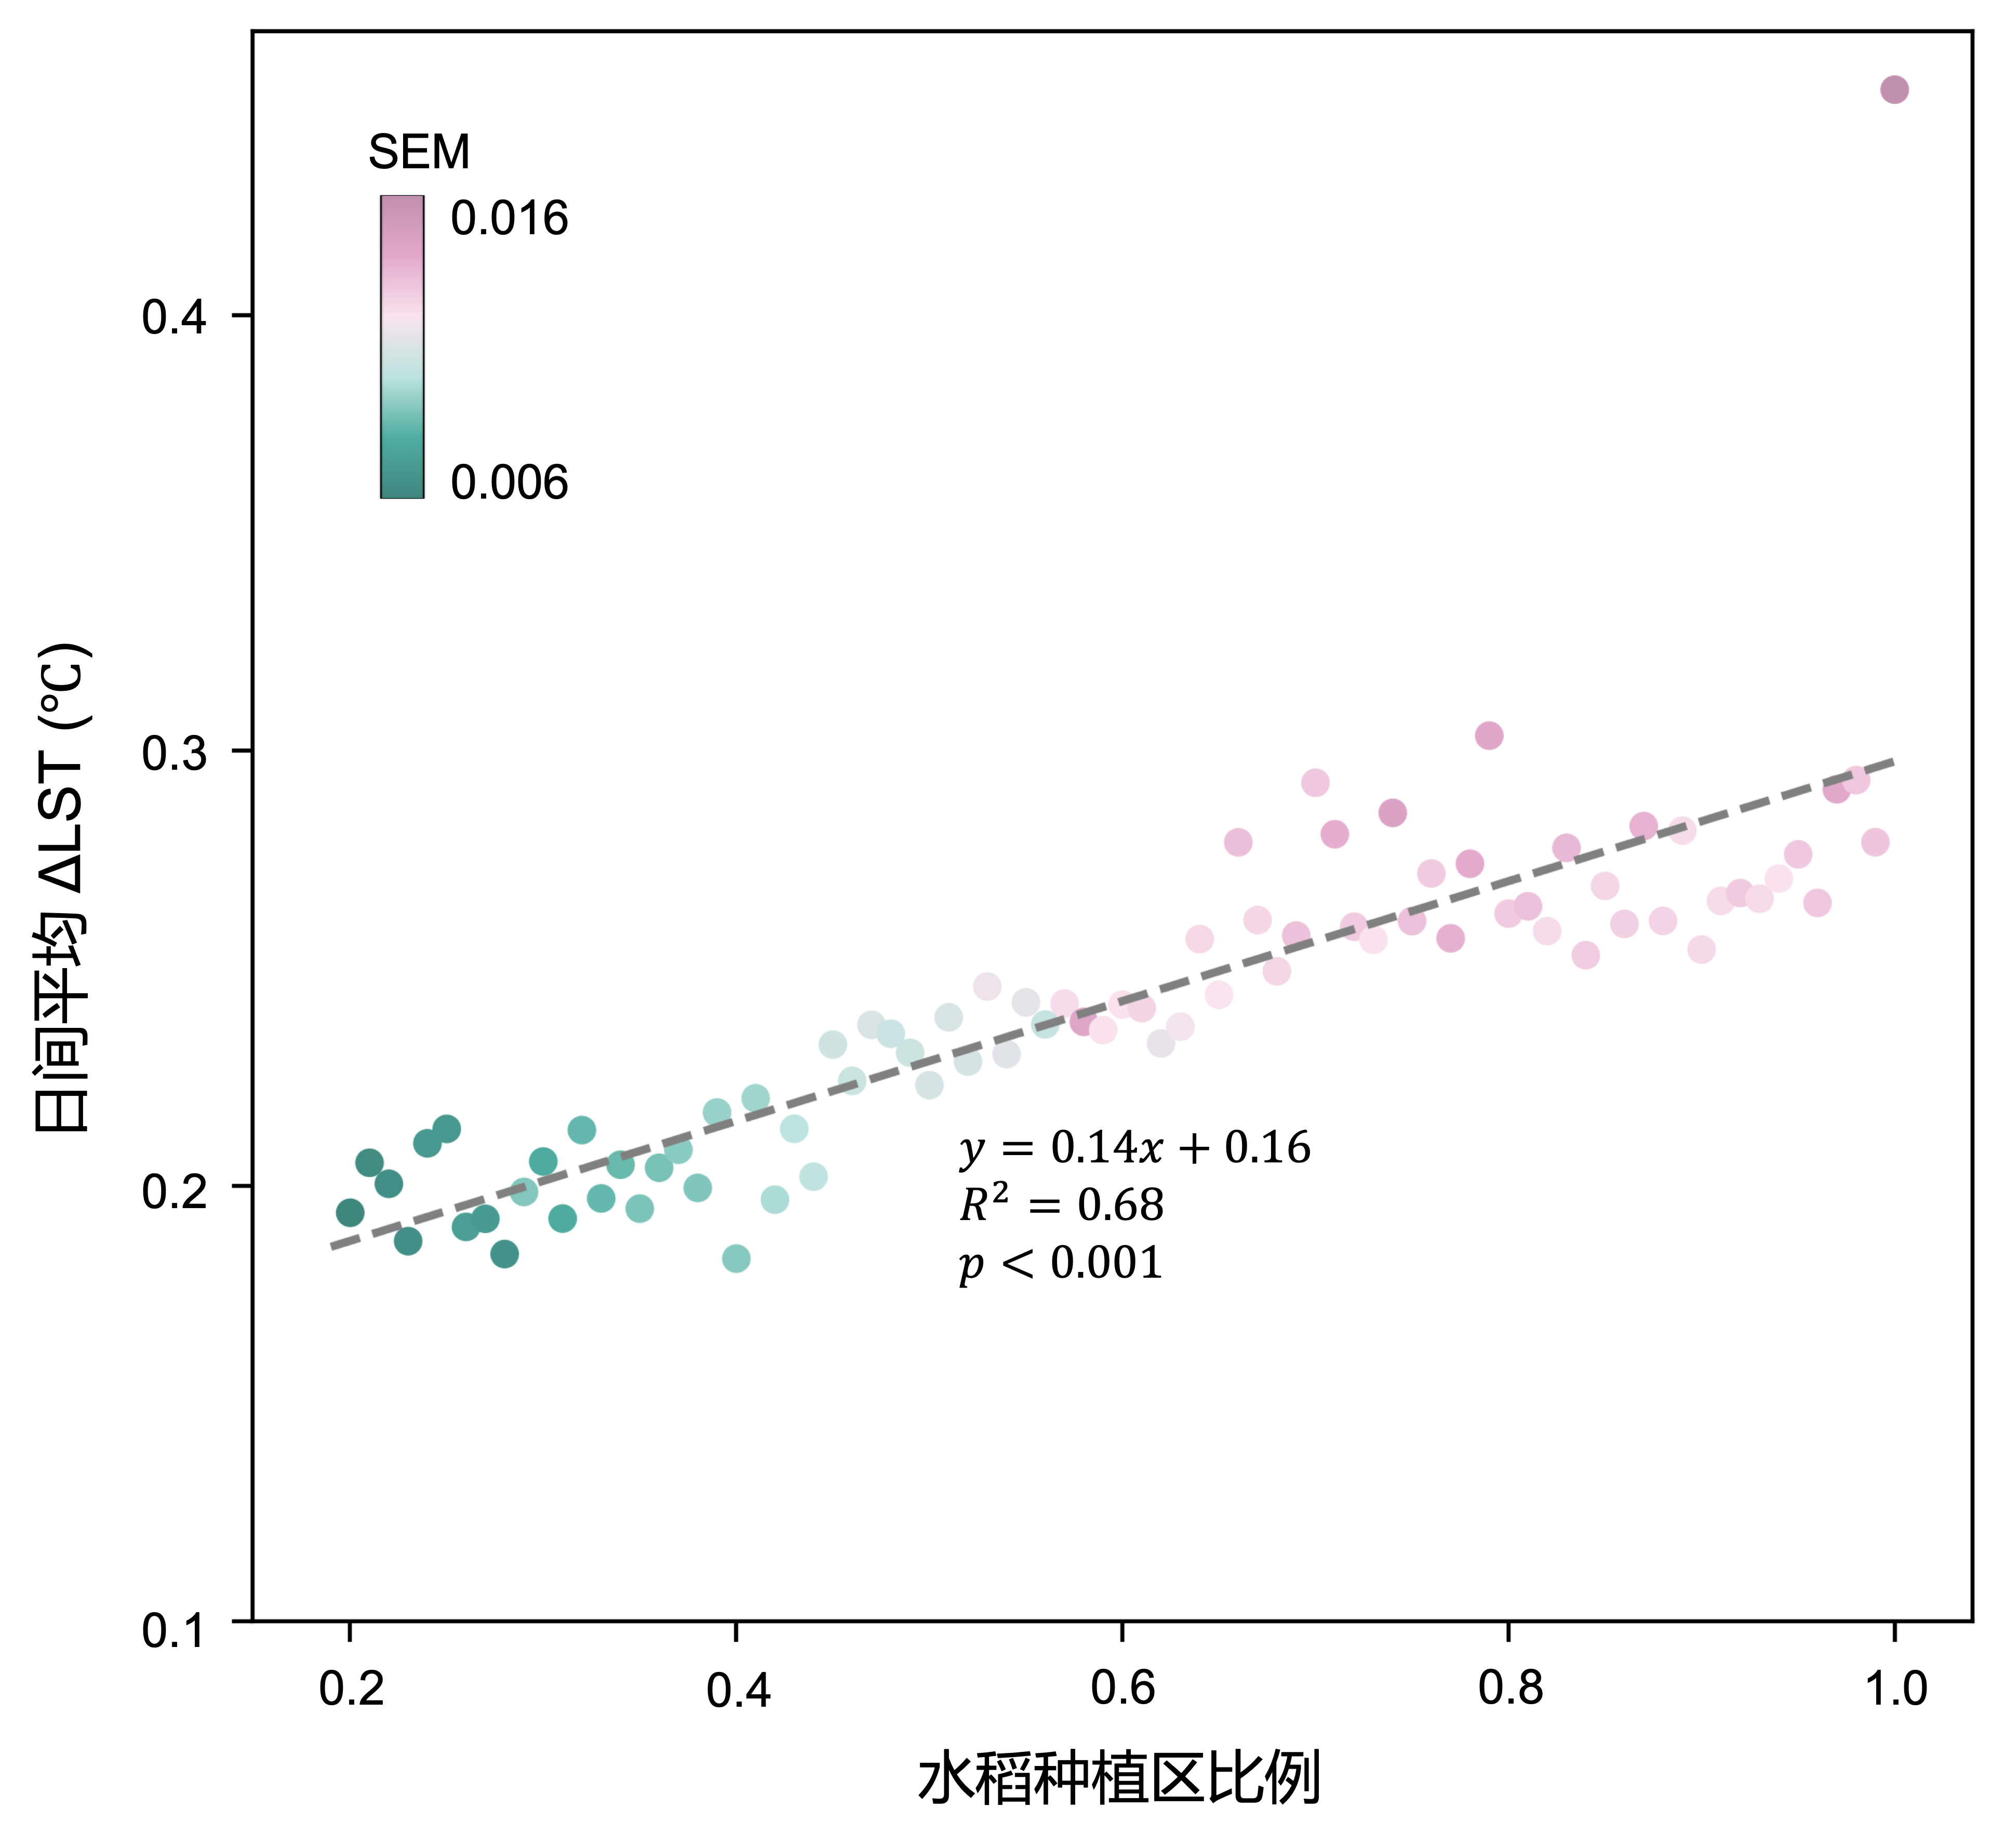
\includegraphics[width=0.7\linewidth]{figure/chapter4/paddy_proportion.png}
    \bicaption[日间 $\Delta \mathrm{LST}$ 与十公里网格内水稻种植区比例的关系]
    {日间 $\Delta \mathrm{LST}$ 与十公里网格内水稻种植区比例的关系。每个点表示一个十公里网格内水稻种植区比例分组的多年平均值，点的颜色表示 SEM。}
    [Relationship between $\Delta \mathrm{LST}$ and Paddy Proportion]
    {Relationship between $\Delta \mathrm{LST}$ and Paddy Proportion. Each point represents the multi-year mean of a Paddy Proportion bin, and the marker color denotes SEM.}
    \label{fig:proportion_regression}
\end{figure}

基于约 $10~\mathrm{km}\times10~\mathrm{km}$ 网格的统计结果表明，日间 $\Delta \mathrm{LST}$ 总体随十公里网格内水稻种植区比例的增加而增大（图 \ref{fig:proportion_regression}）。
线性回归结果显示，十公里网格内水稻种植区比例与日间 $\Delta \mathrm{LST}$ 呈显著正相关关系。%（$y=0.14x+0.16$，$R^2=0.68$，$p<0.001$）。
%由于 $P_{\mathrm{paddy}}$ 采用 0--1 之间的小数表示，
十公里网格内水稻种植区比例每增加 0.01（即增加 1 个百分点），日间 $\Delta \mathrm{LST}$ 平均增加约 $0.0014~^{\circ}\mathrm{C}$。

上述十公里网格内水稻种植区比例与日间 $\Delta \mathrm{LST}$ 的正相关关系说明，水稻种植区的日间降温强度与局地下垫面中的水稻面积占比密切相关。
当十公里网格内水稻种植区比例较高时，田面水、湿润土壤和水稻冠层构成的复合下垫面占据较大面积，其蒸发和冠层蒸腾对潜热通量的贡献能够在局地范围内形成较为一致的热力特征，从而使水稻种植区相对于周边非水稻耕地的日间低温信号更加明显。
在十公里网格内水稻种植区比例较低的网格中，水稻种植区下垫面所占份额较小，局地热力背景通常具有更强的异质性，水稻像元的低温信号更容易受到周边非水稻下垫面的影响，因而平均 $\Delta \mathrm{LST}$ 相对较弱。

日间 $\Delta \mathrm{LST}$ 与十公里网格内水稻种植区比例的正相关关系说明，水稻种植区降温效应不仅与水稻种植区的存在有关，还与其在局地下垫面中的相对覆盖程度有关。
% 不同稻作区之间水稻覆盖比例的差异，可能构成全球水稻种植区日间降温强度空间异质性的一个重要来源。
% 该结果也提示，在评估水稻种植区面积变化的地表温度效应时，除关注面积变化总量外，还需要考虑其是否改变了局地范围内水稻下垫面的相对占比。
从土地系统变化角度看，水稻种植区面积扩张或收缩对地表温度的影响不仅取决于面积变化本身，还取决于局地景观中水稻种植区水—植被—土壤复合下垫面的相对主导程度。

\section{水稻种植区降温效应随水稻种植区规模的变化}
\label{sec:paddy_size}

本节分析水稻种植区规模（Paddy Size）对日间 $\Delta \mathrm{LST}$ 的影响，以表征水稻种植区的空间连续性对水稻种植区降温强度的影响。
\begin{figure}[htbp]
    \centering
    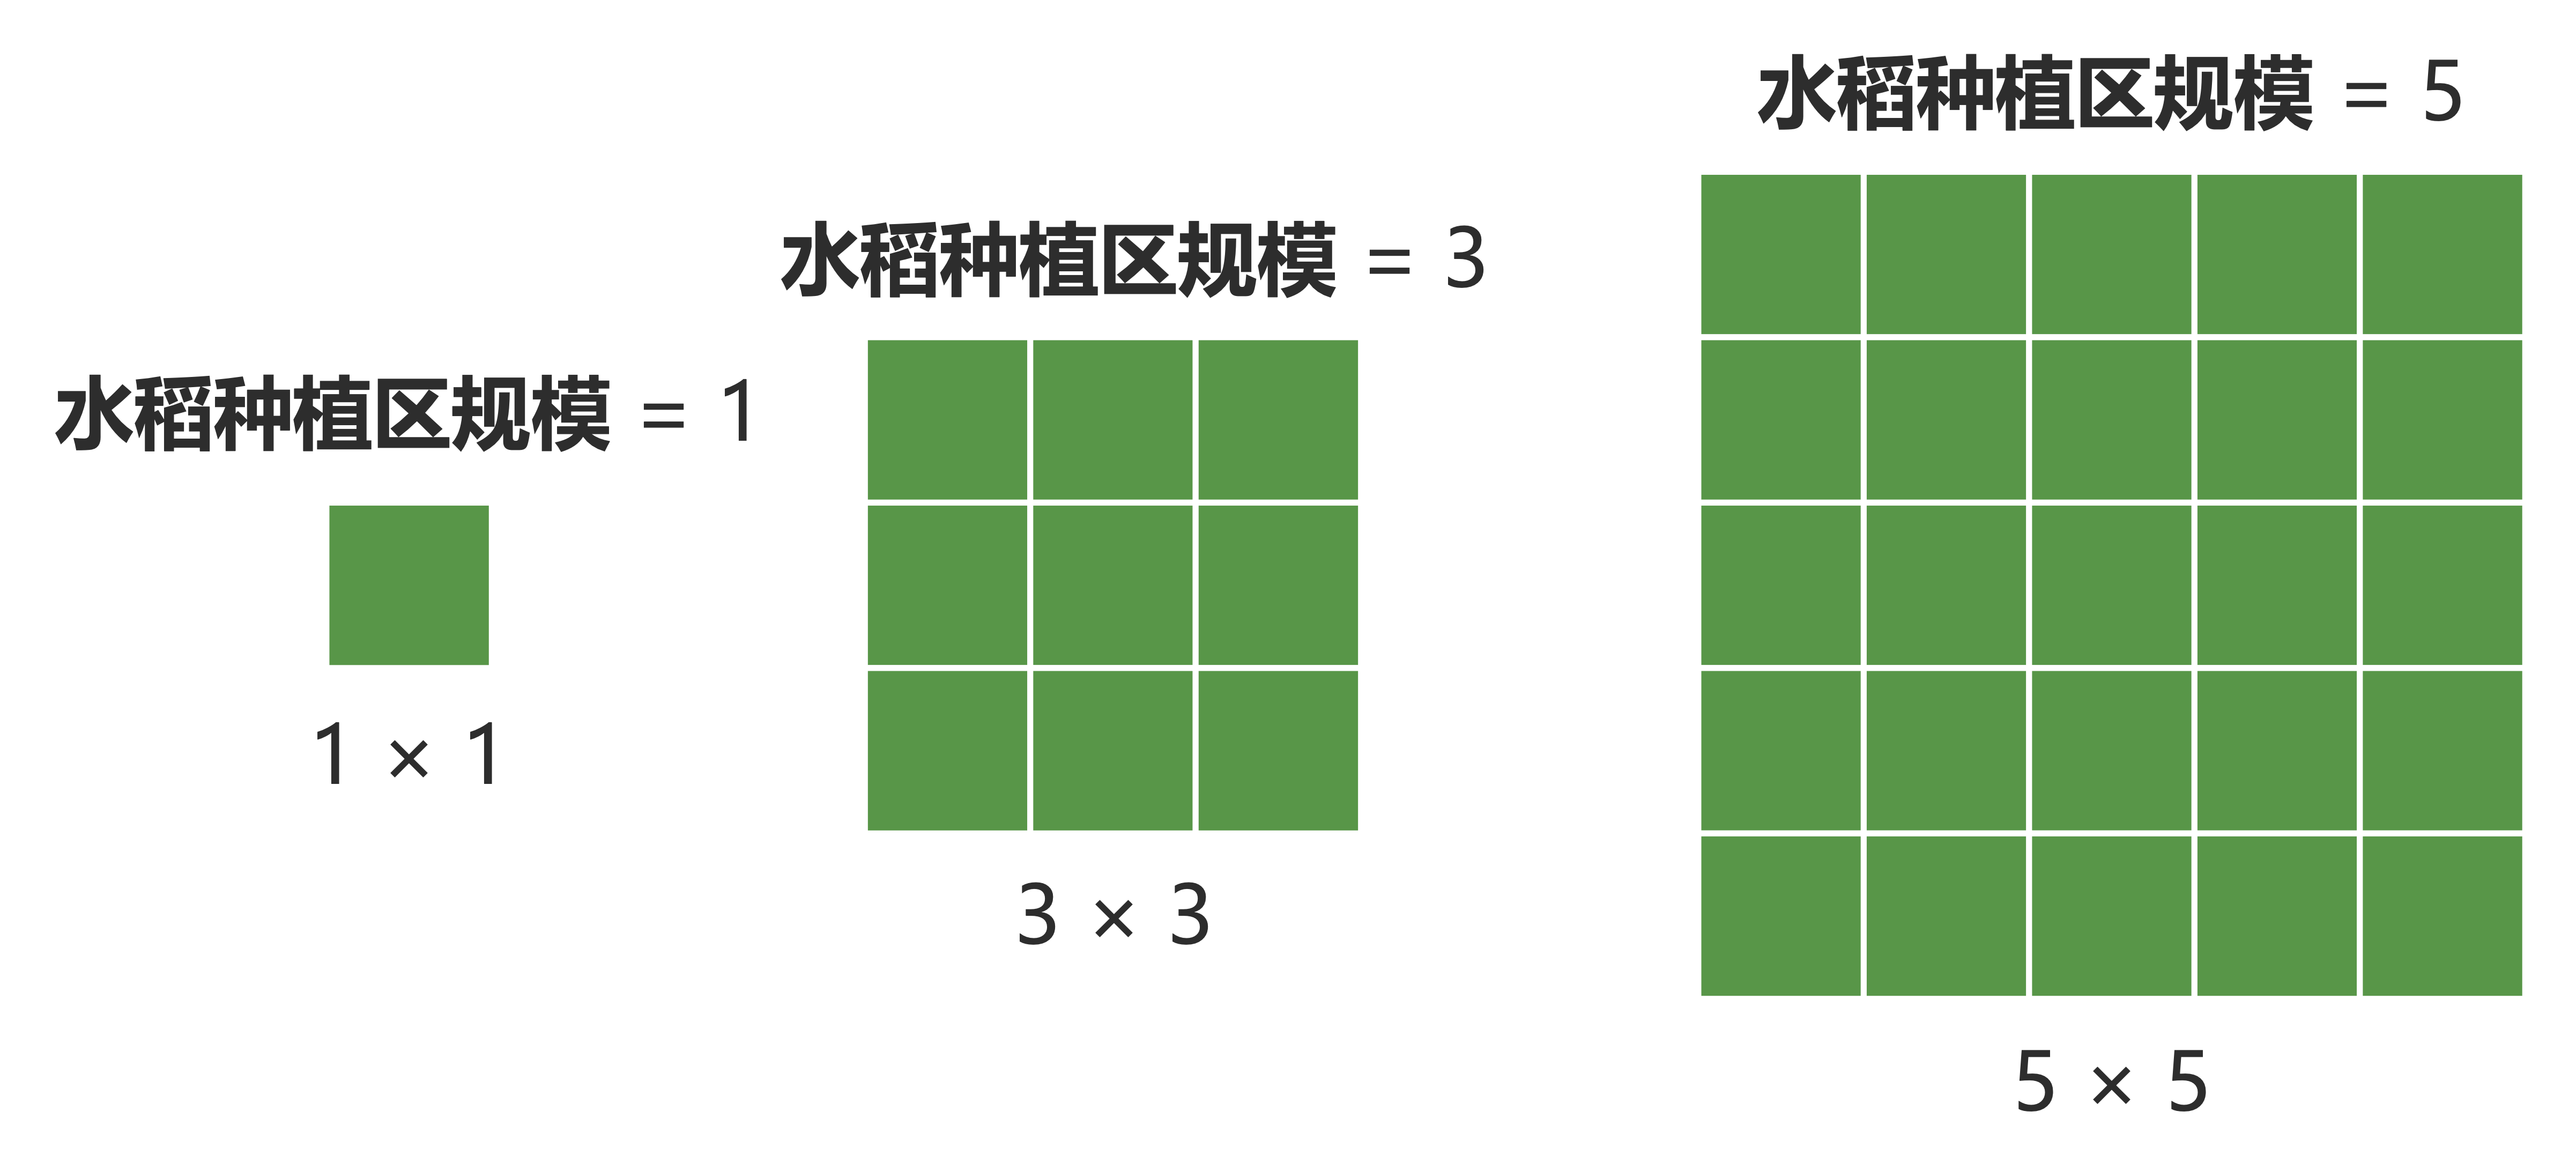
\includegraphics[width=0.6\linewidth]{figure/chapter4/NPL_definition_b.png}
    \bicaption[水稻种植区规模示意图]
    {水稻种植区规模示意图。
    水稻种植区规模定义为由空间连续的水稻像元构成的正方形窗口边长，并以 MODIS 像元数表示。规模 $n$ 对应由 $n \times n$ 个连续 MODIS 像元组成的水稻种植区。
    }
    [Schematic illustration of Paddy Size]
    {Schematic illustration of Paddy Size.
    Paddy Size is defined as the side length of a square window composed of spatially contiguous rice pixels and is expressed as the number of MODIS pixels along one side.
    Paddy Size $n$ corresponds to a rice-growing area consisting of $n \times n$ contiguous MODIS rice pixels.
    }
    \label{fig:NPL_definition_b}
\end{figure}
本研究以连续水稻种植区像元构成的正方形窗口边长表征水稻种植区连片规模。当规模为 $n$ 时，表示由 $n \times n$ 个连续 MODIS 水稻种植区像元构成的正方形区域（图 \ref{fig:NPL_definition_b}）。例如，规模为 1 对应约 $500~\mathrm{m} \times 500~\mathrm{m}$ 的连续水稻覆盖范围，规模为 5 对应约 $2.5~\mathrm{km} \times 2.5~\mathrm{km}$ 的连续水稻覆盖范围。%需要指出的是，该指标衡量的是基于 500 m 水稻像元所能形成的方形连片尺度，而非形状不规则的水稻种植区斑块的实际总面积。

结果显示，日间平均 $\Delta \mathrm{LST}$ 随水稻种植区连片规模增大而持续增强（图 \ref{fig:paddy_size_dlst}）。随着规模由 1 增加至 11，即连续水稻覆盖范围由约 $500~\mathrm{m} \times 500~\mathrm{m}$ 扩大至约 $5.5~\mathrm{km} \times 5.5~\mathrm{km}$，日间平均 $\Delta \mathrm{LST}$ 由约 $0.13~^{\circ}\mathrm{C}$ 增加至约 $0.43~^{\circ}\mathrm{C}$。
该结果表明，在本研究的遥感观测尺度下，空间连续性较高的水稻种植区表现出更强的日间降温特征。

以往区域研究表明，水稻种植区的扩张及空间分布变化能够通过生物物理过程影响地表温度，其效应强度同时受到水稻种植区空间集聚程度和背景地表条件的影响 \cite{Liu2022AgForMet}。
本研究中，随着连片规模增大，水稻种植区内部远离水稻与非水稻耕地边界的区域比例提高，受边缘混合、邻近异质地表干扰及 LST 像元混合的影响相对减弱，使连续湿润下垫面的水分条件、植被覆盖和地表能量分配特征能够在遥感 LST 中得到更充分的表达。相比之下，不同连片规模下的夜间 $\Delta \mathrm{LST}$ 均接近 0，且未表现出随连片规模增大而增强的变化趋势，进一步说明连片规模对水稻种植区温度效应的影响主要体现在日间。

\begin{figure}[htbp]
    \centering
    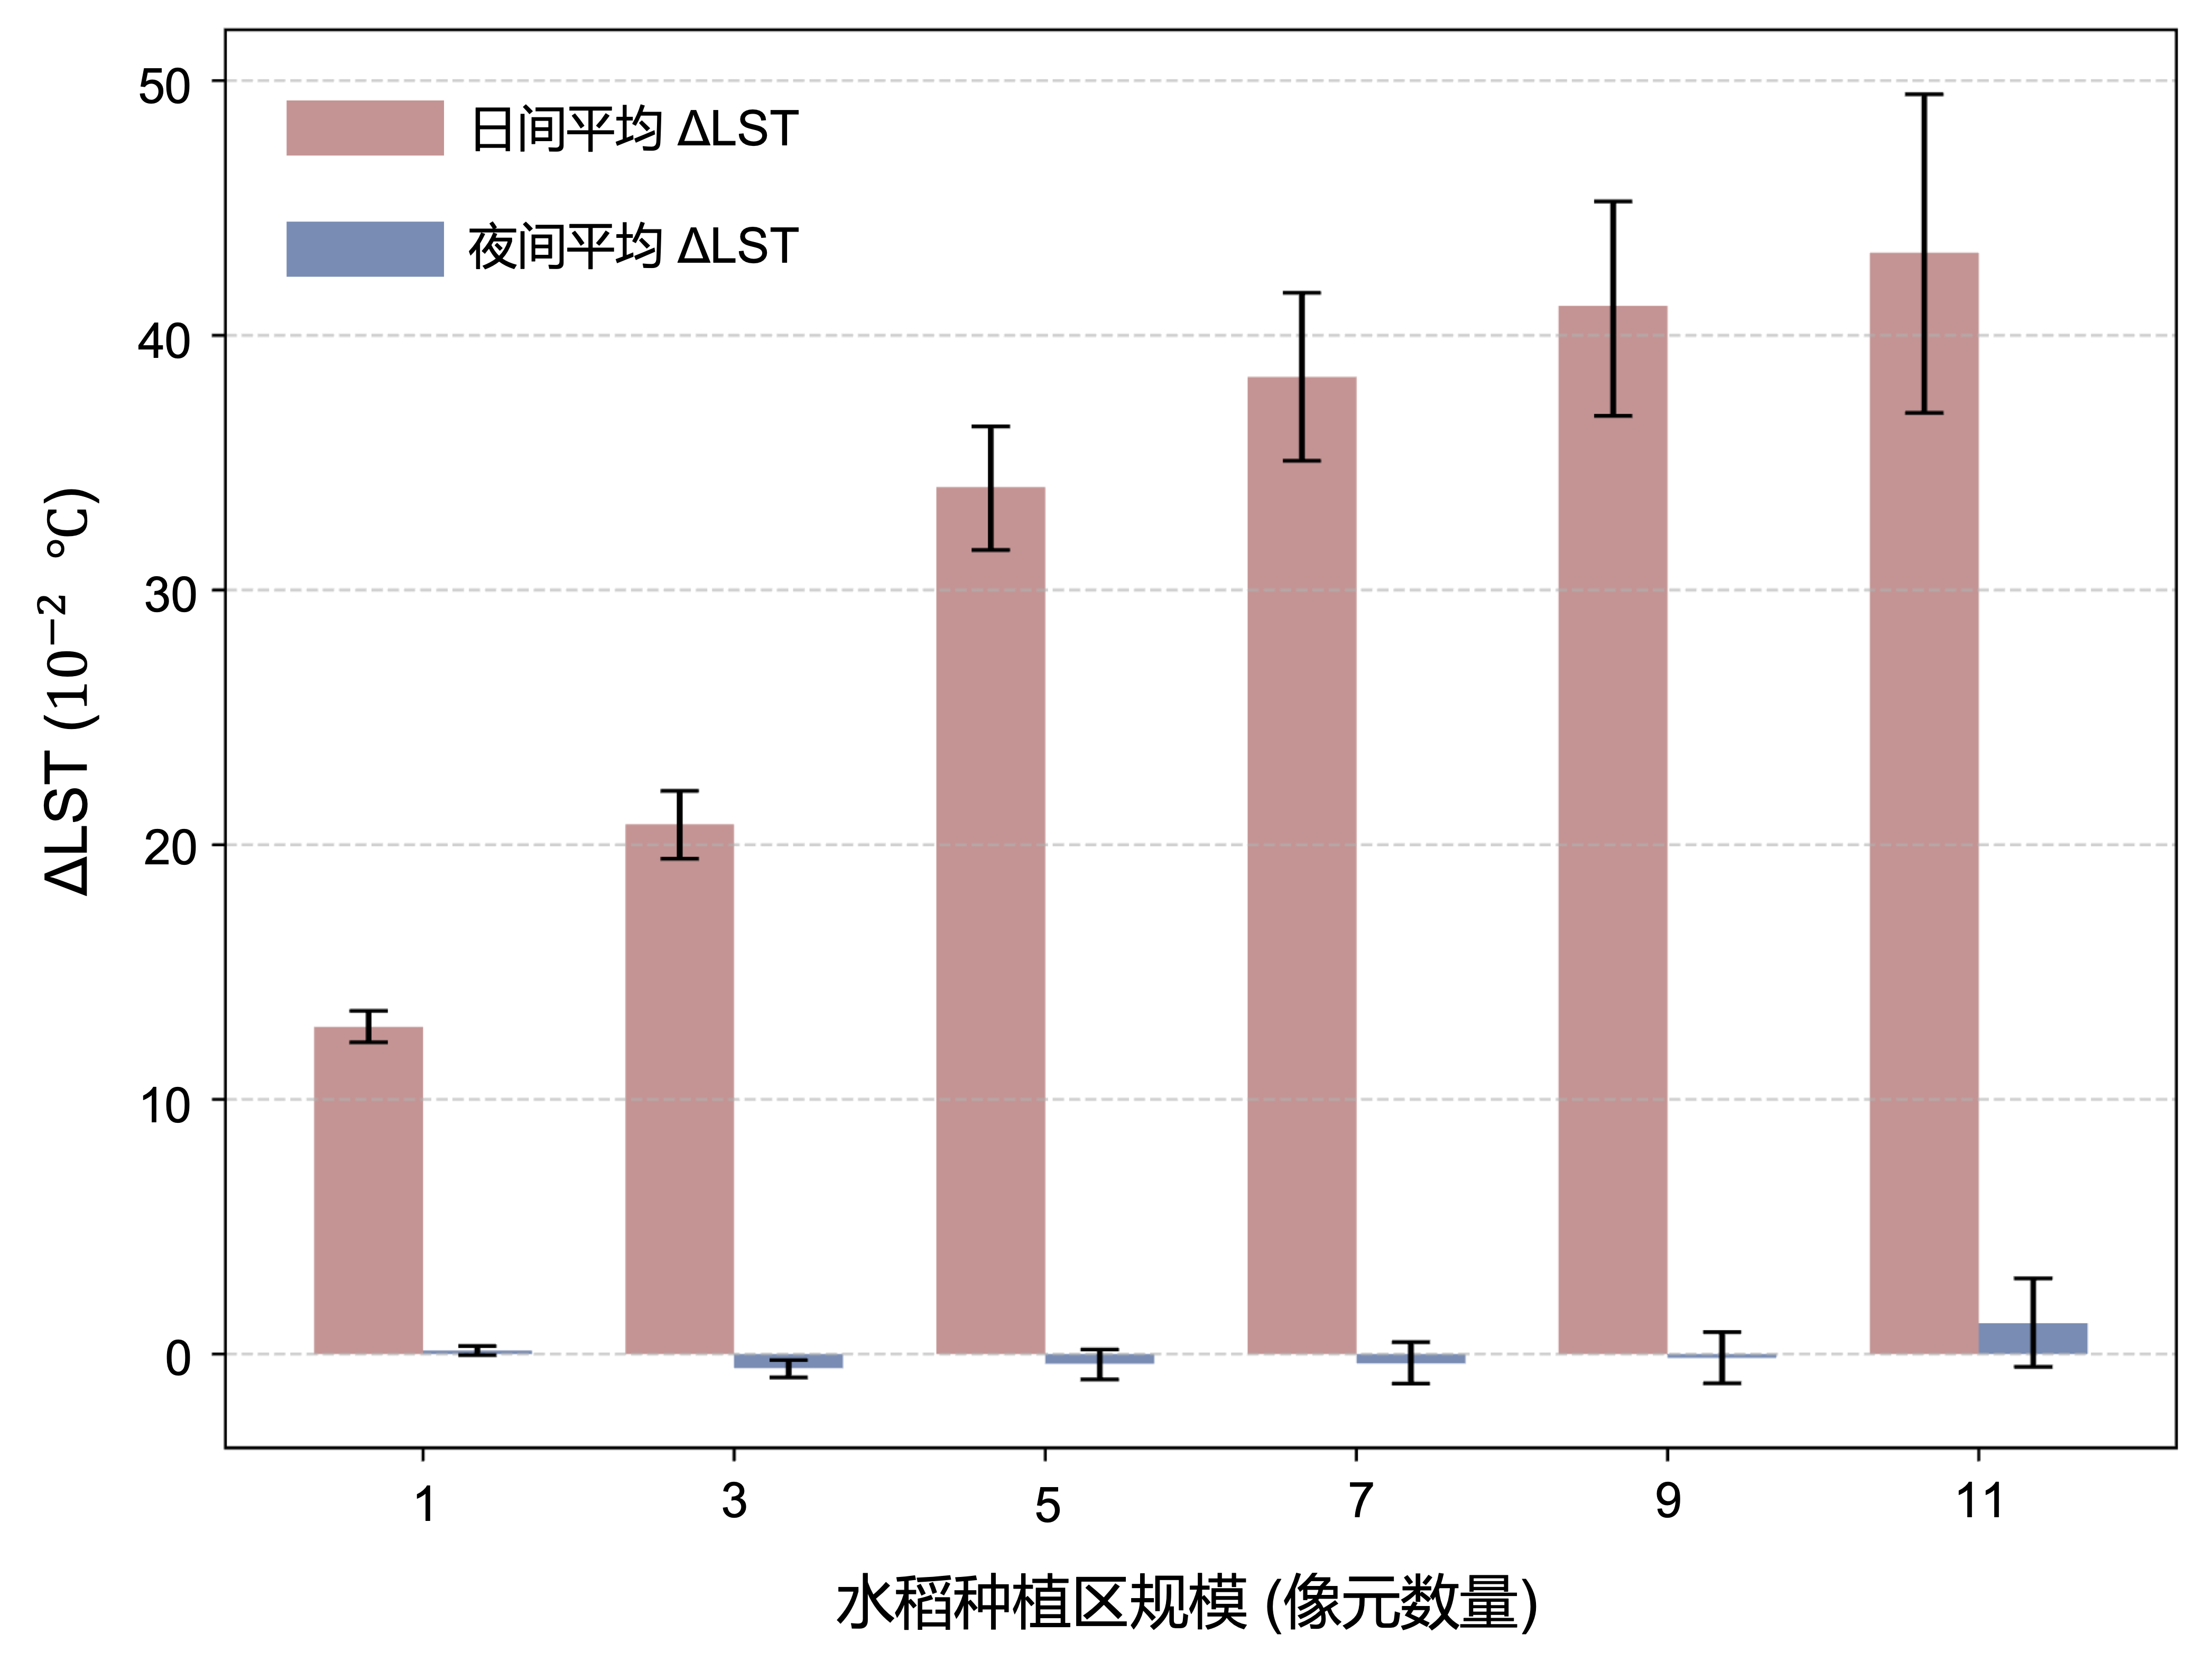
\includegraphics[width=0.7\linewidth]{figure/chapter4/paddy_size.png}
    \bicaption[不同水稻种植区规模的平均 $\Delta \mathrm{LST}$]
    {不同水稻种植区规模的平均 $\Delta \mathrm{LST}$。
    水稻种植区规模以由连续水稻像元构成的正方形窗口的边长表示，并以单边 MODIS 像元数计。规模 $n$ 对应由 $n \times n$ 个连续 MODIS 水稻像元组成的种植区。误差线表示 95\% 置信区间。}
    [Mean $\Delta \mathrm{LST}$ across different Paddy Sizes]
    {Mean $\Delta \mathrm{LST}$ across different Paddy Sizes. Paddy Size is represented by the side length of a square window composed of contiguous rice pixels and is expressed as the number of MODIS pixels along one side. Paddy Size $n$ corresponds to a rice-growing area consisting of $n \times n$ contiguous MODIS rice pixels. Error bars denote 95\% confidence intervals.}
    \label{fig:paddy_size_dlst}
\end{figure}

\section{不同非水稻耕地梯度环带的地表温度变化}
\label{sec:npl}

为分析水稻种植区边界外邻近非水稻耕地地表温度随距离的变化，本研究构建非水稻耕地梯度环带（Non-Paddy Ladder, NPL），按照与水稻种植区边界的像元距离，将周边非水稻耕地划分为一系列空间比较单元（图 \ref{fig:NPL_definition_c}）。其中，$NPL_d$ 表示水稻种植区边界外第 $d$ 个像元层级、宽度为 1 个 MODIS 像元的非水稻耕地环带；$NPL_{d_1-d_2}$ 表示由第 $d_1$ 至第 $d_2$ 个环带共同组成的非水稻耕地区域。下标所表示的距离均以 MODIS 像元为单位，单个像元的空间分辨率约为 500 m。

\begin{figure}[htbp]
    \centering
    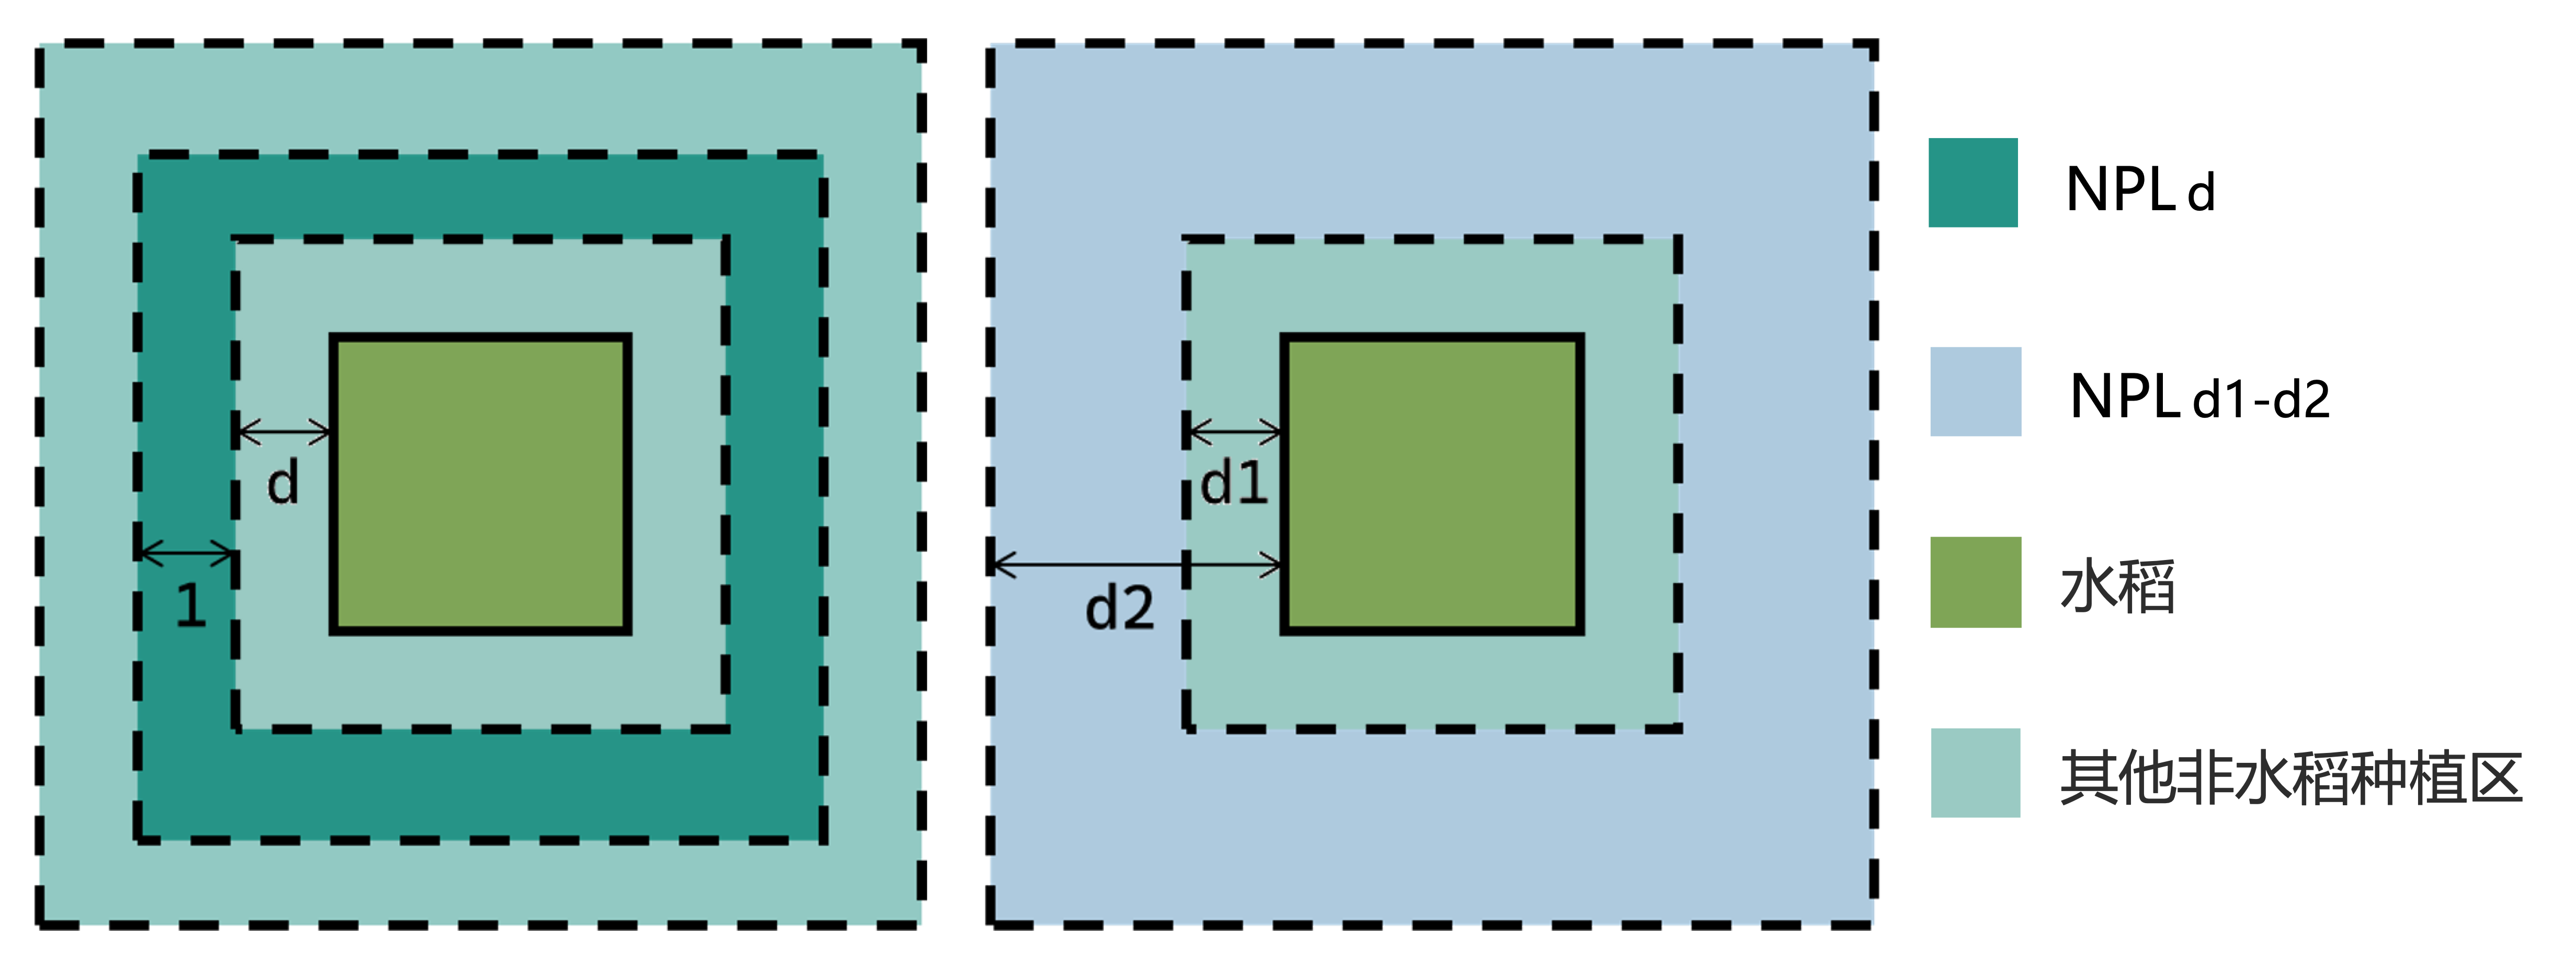
\includegraphics[width=0.9\linewidth]{figure/chapter4/NPL_definition_c.png}
    \bicaption[非水稻耕地梯度环带示意图]
    {非水稻耕地梯度环带示意图。
    $NPL_d$ 表示距水稻种植区边界第 $d$ 个 MODIS 像元处、宽度为 1 个像元的非水稻环带；$NPL_{d_1-d_2}$ 表示距水稻种植区边界 $d_1$ 至 $d_2$ 个像元之间的非水稻耕地区域。
    }
    [Schematic illustration of Non-Paddy Ladder]
    {Schematic illustration of Non-Paddy Ladder.
    $NPL_d$ denotes the one-pixel-wide square-shaped ring of non-paddy cropland at a distance of $d$ MODIS pixels from the boundary of rice growing area, and $NPL_{d_1-d_2}$ denotes non-paddy cropland between $d_1$ and $d_2$ MODIS pixels from the boundary.
    }
    \label{fig:NPL_definition_c}
\end{figure}

结果表明，靠近水稻种植区边界的 NPL 展现出较小的日间 $\Delta \mathrm{LST}$；随着距水稻种植区边界的像元距离增加，$\Delta \mathrm{LST}$ 逐渐增大并趋于稳定（图 \ref{fig:npl_spillover_gradient}）。
即靠近水稻种植区的 NPL 具有相对较低的地表温度，其地表温度随距水稻种植区边界距离增加而逐渐升高，随后趋于相对稳定的背景水平。
不同水稻种植区规模下的 NPL 曲线均表现出 $\Delta \mathrm{LST}$ 随距水稻种植区边界距离增加而逐渐升高并趋于稳定的特征。较大连片水稻种植区所对应的 $\Delta \mathrm{LST}$ 整体较高，与第 \ref{sec:paddy_size} 节所述更大规模的水稻种植区日间降温更强的现象一致。

上述温度梯度表明，水稻种植区降温影响可能并非完全局限于其内部，而延伸至邻近非水稻耕地。水稻种植区内田面水蒸发、湿润土壤蒸发和冠层蒸腾能够增强潜热交换，形成相对冷湿的局地环境；水稻种植区与周边非水稻耕地之间的温度和水分差异，可能通过近地层水汽输送及热量交换影响边界附近非水稻耕地的地表能量状态。随着距水稻种植区边界的距离增加，这种邻近影响逐渐减弱，非水稻耕地地表温度逐渐趋近于相对稳定的背景水平。

\begin{figure}[htbp]
    \centering
    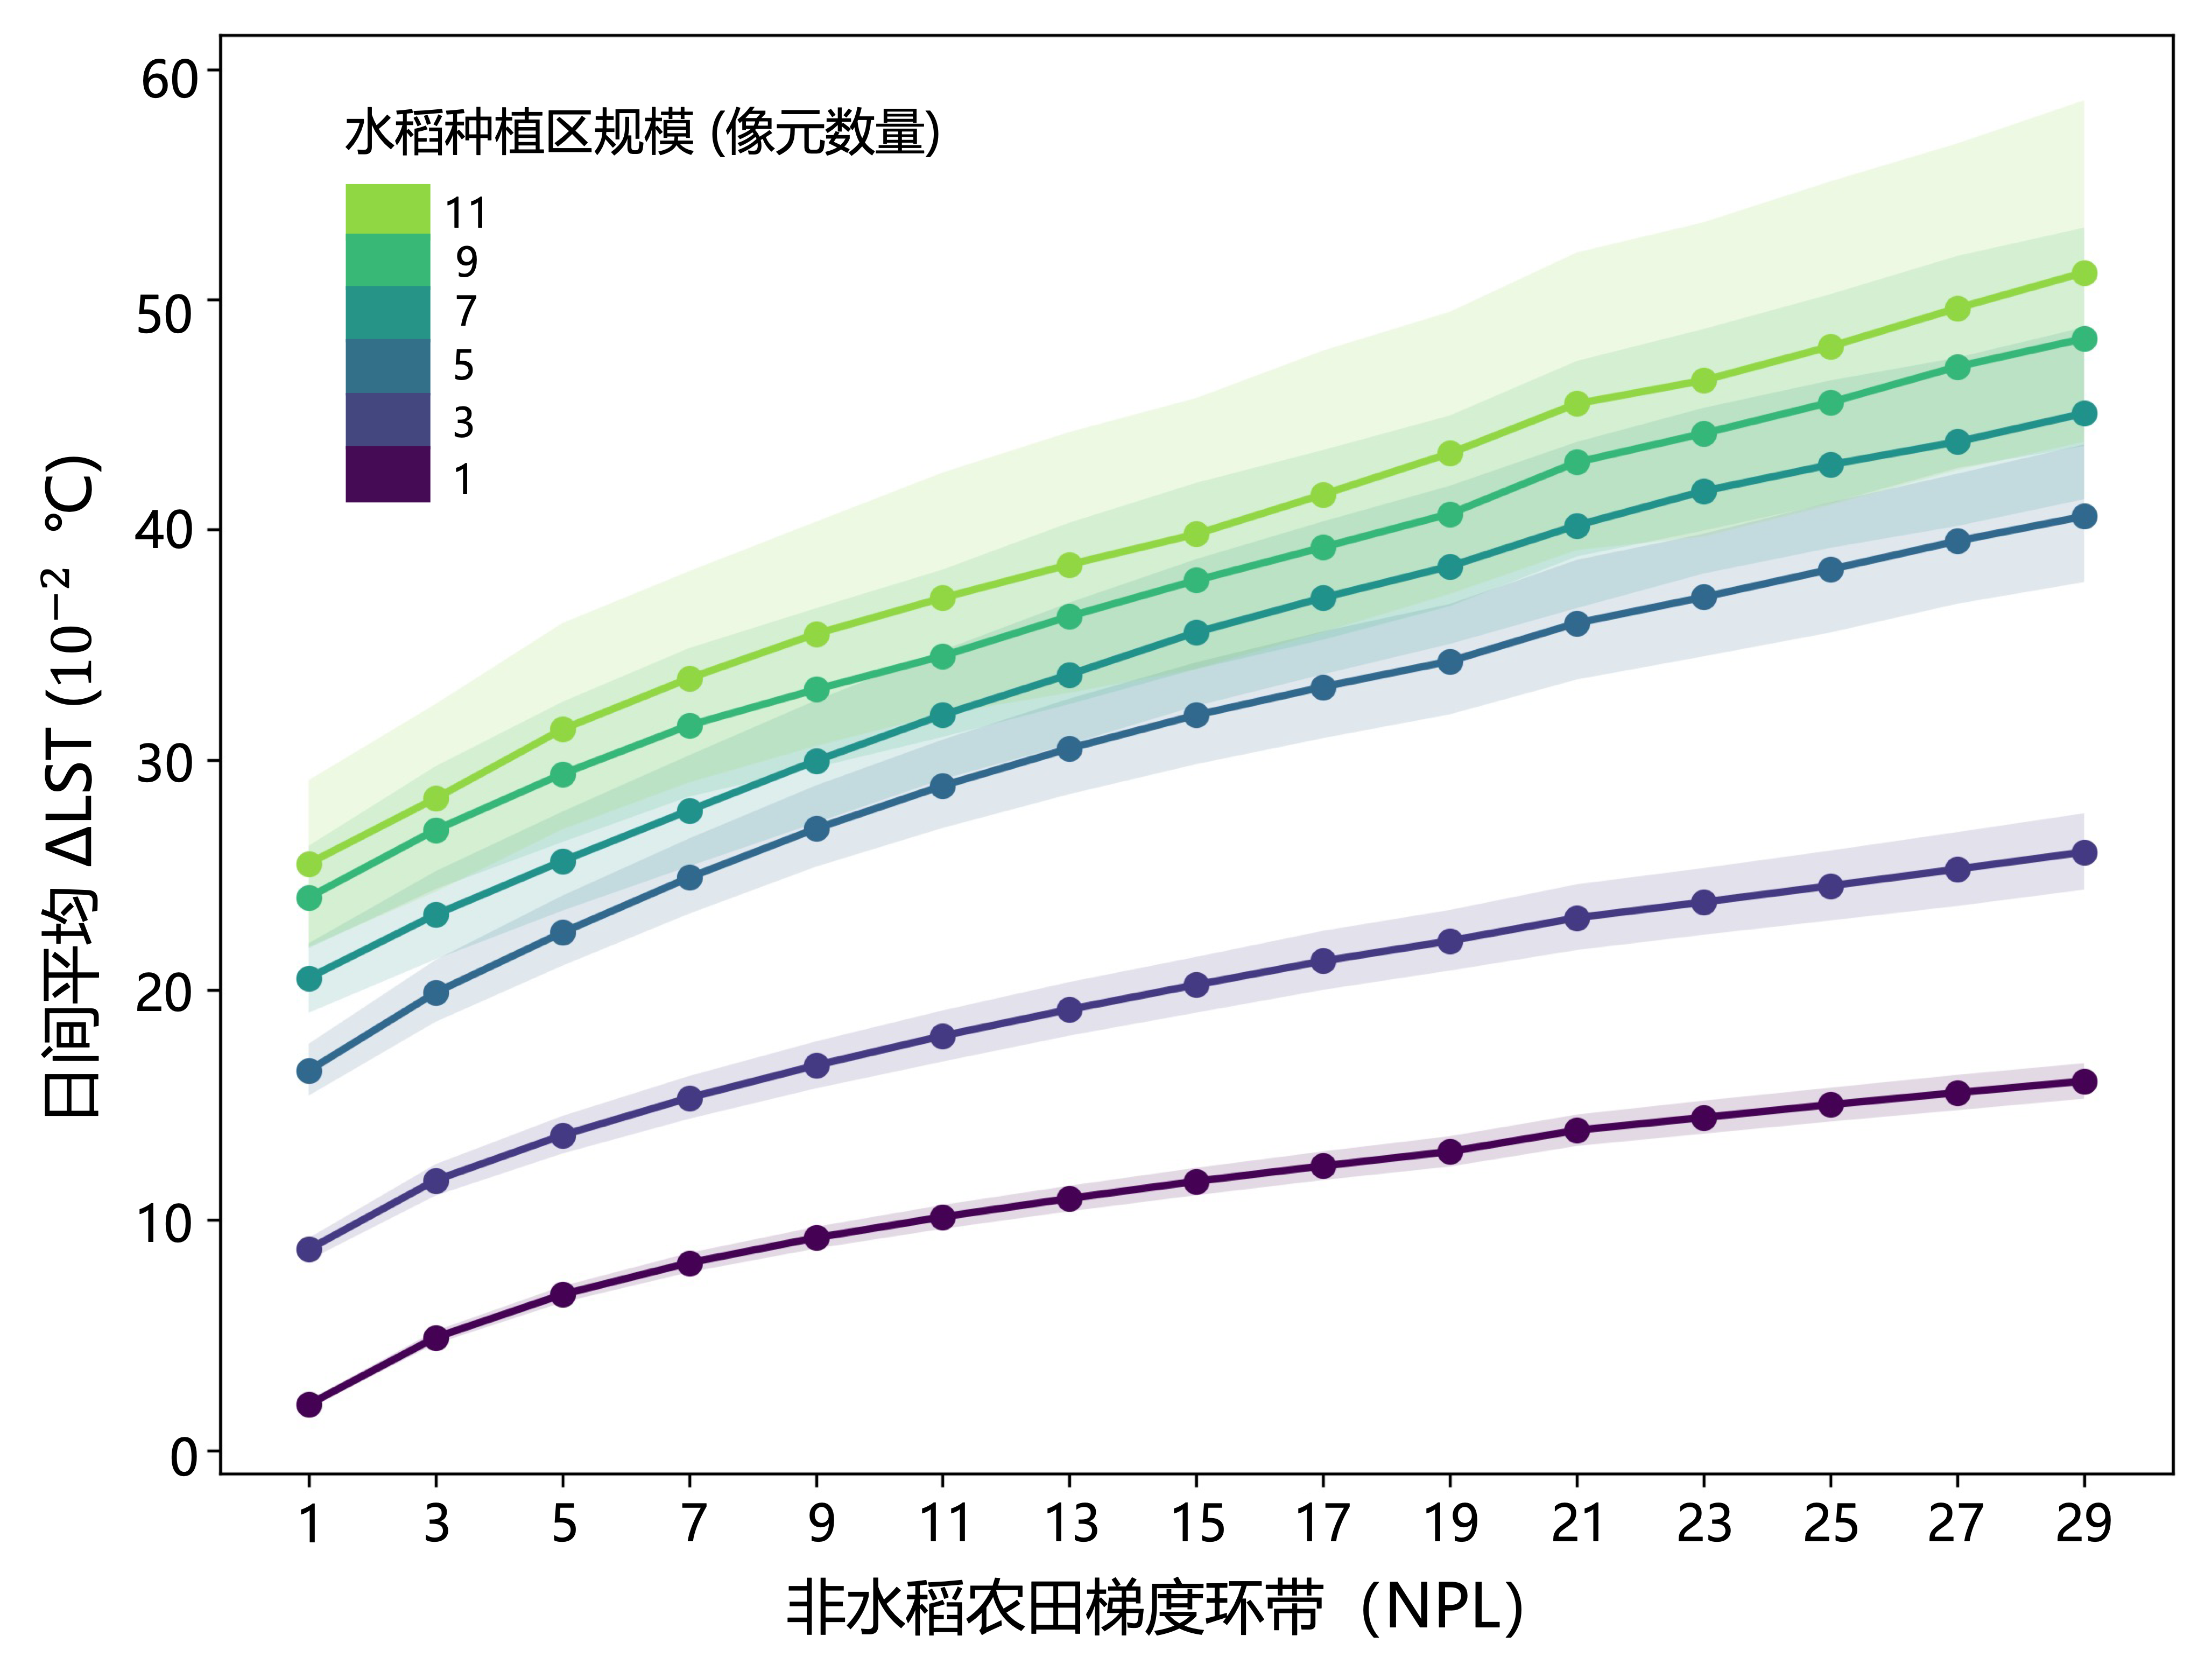
\includegraphics[width=0.8\linewidth]{figure/chapter4/paddy_NPL.png}
    \bicaption[水稻种植区降温的外溢效应]
    {水稻种植区降温的外溢效应。
    横轴中的数字 $k$ 表示非水稻耕地梯度环带 $NPL_k$ 的下标。纵轴为日间平均 $\Delta \mathrm{LST}$。
    不同颜色表示不同规模的水稻种植区。
    带标记的曲线表示均值，阴影带表示 95\% 置信区间。
    %曲线用于表征邻近非水稻农田地表温度差异随距水稻种植区边界距离增加的变化。
    }
    [Spillover effect of paddy cooling]
    {Spillover effect of paddy cooling. 
    The number $k$ on the horizontal axis denotes the subscript of the non-paddy ladder $NPL_k$. The y-axis denotes daytime $\Delta \mathrm{LST}$. 
    Different colors indicate paddy rice areas of varying sizes. 
    Lines with markers show the means, and shaded ribbons indicate the 95\% confidence intervals.
    %The curves characterize how the LST difference in neighboring non-paddy croplands changes with distance from rice-growing-area boundaries.
    }
    \label{fig:npl_spillover_gradient}
\end{figure}

降温外溢现象也为 $\Delta \mathrm{LST}$ 的非水稻种植区对照样本的选取提供了参考依据。
如果直接采用紧邻水稻种植区边界的非水稻耕地作为对照，其地表温度可能因受到邻近水稻种植区低温环境影响而偏低，从而减小 $\mathrm{LST}{\mathrm{non\text{-}paddy}}$，低估水稻种植区相对于背景非水稻耕地的降温强度。
因此，在前述总体 $\Delta \mathrm{LST}$ 均值估计（第\ref{sec:overall_dlst}节）以及关于十公里内水稻种植区比例（第\ref{sec:paddy_proportion}节）和水稻种植区规模（第\ref{sec:paddy_size}节）对 $\Delta \mathrm{LST}$ 的影响，以及后续 $\Delta \mathrm{LST}$ 生长季动态（第\ref{sec:paddy_dos}节）等分析中，本研究均采用 $NPL_{10-30}$ 作为默认对照，以降低近距离温度梯度对 $\Delta \mathrm{LST}$ 估计的影响。

总体而言，邻近非水稻耕地地表温度随距离增加而升高并趋于稳定的现象，为水稻种植区降温的外溢效应提供了遥感观测证据，也为将水稻种植区空间配置、农田水分管理和农业适应性降温效应纳入综合土地系统研究提供了依据。
%在热风险较高、农田与建设用地交错分布或灌溉水分条件允许的区域，水稻种植区空间布局对局地地表热环境的调节作用具有进一步评估价值。
\clearpage

\section{水稻种植区降温效应的生长季动态}
\label{sec:paddy_dos}

本节进一步在不同水稻种植区规模下分析日间 $\Delta \mathrm{LST}$ 随生长季日序的变化，刻画水稻种植区降温效应的季内动态，并比较不同水稻种植区规模之间的差异。
% DOS 定义
本研究将逐日 $\Delta \mathrm{LST}$ 从自然日期坐标转换至相对生长季进程坐标，以减少不同地区播栽时间和复种制度差异造成的时间错配，并提高水稻种植区降温效应季内动态的跨区域可比性。%基于 GlobalRice500 提供的逐像元水稻生长季边界，
%全球稻区在播栽日期、生长季长度和复种制度上差异显著。热带多熟稻区、亚热带双季稻区和温带单季稻区可能在完全不同的自然月份进入相似的生育阶段；同一自然月份在不同区域也可能对应移栽、分蘖、抽穗、成熟或收获后等不同阶段。若仅依据固定月份或自然年日序组织 LST 比较，同一时间窗口在不同地区可能对应不同的水稻生育阶段，从而削弱 $\Delta \mathrm{LST}$ 与实际水稻生长过程之间的时间对应关系。因此，跨区域分析水稻种植区降温效应的生长季动态，需要将逐日温度差异从自然日期坐标转换到相对生育进程坐标。

\begin{figure}[htbp]
    \centering
    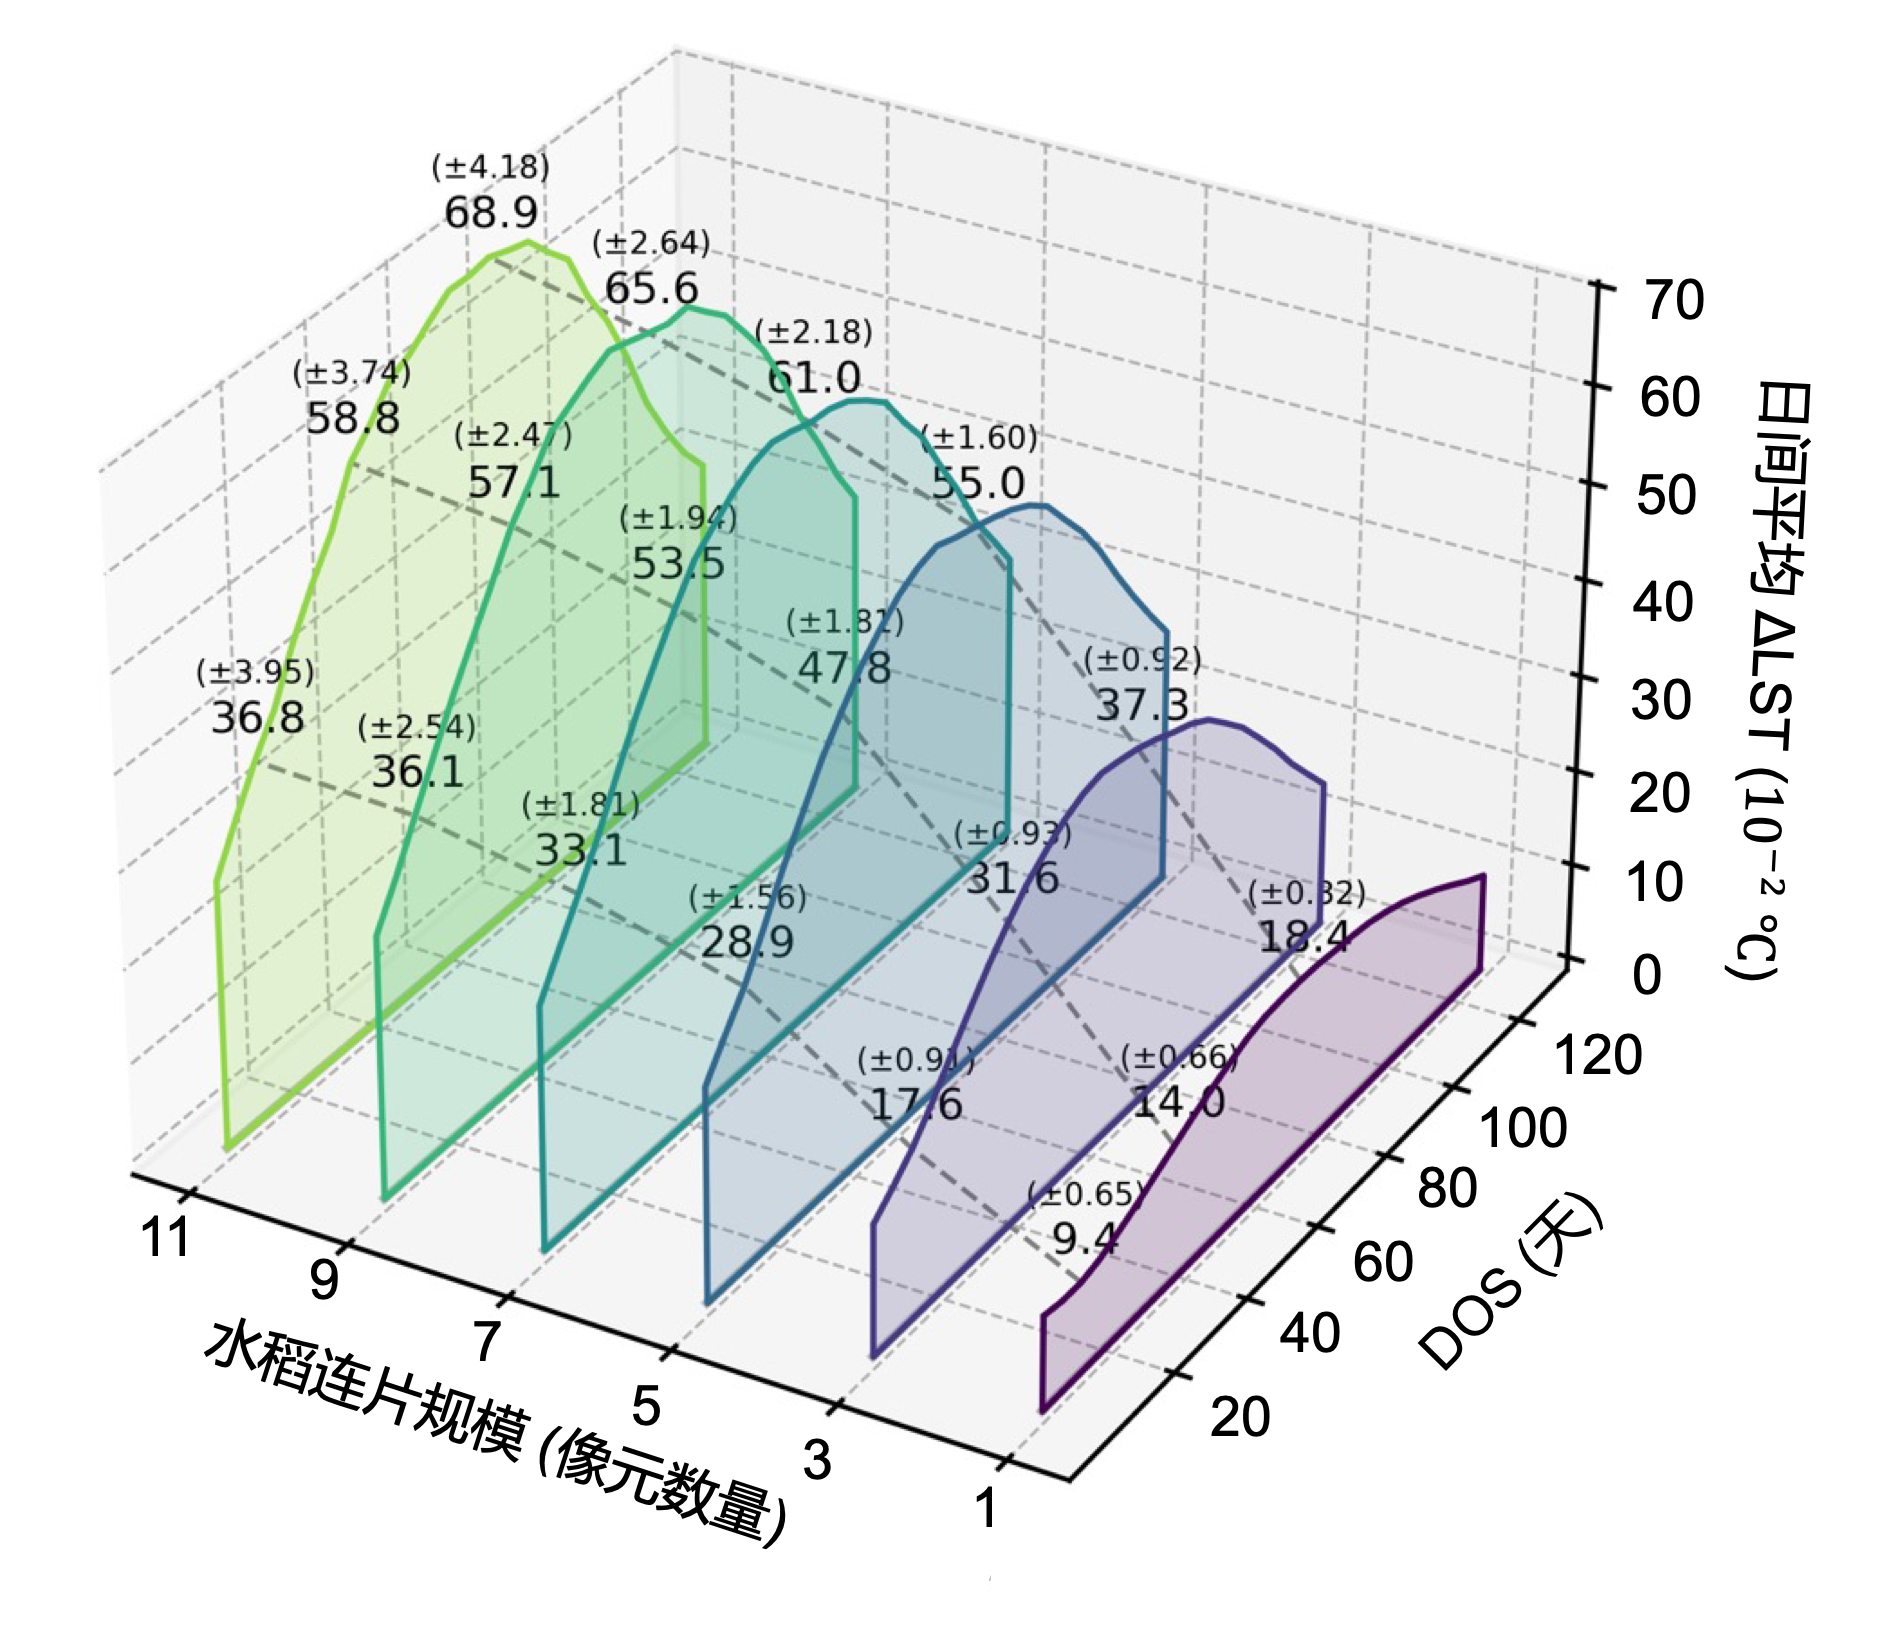
\includegraphics[width=0.7\linewidth]{figure/chapter4/paddy_season.png}
    \bicaption[不同水稻种植区规模的日间 $\Delta \mathrm{LST}$ 生长季动态]
    {不同水稻种植区规模的日间 $\Delta \mathrm{LST}$ 生长季动态。横轴为生长季日序（Day of Season, DOS）；纵轴为日间 $\Delta \mathrm{LST}$。不同颜色的曲线表示不同水稻种植区规模的 $\Delta \mathrm{LST}$ 生长季动态，曲线采用五日滑动平均进行平滑。}
    [Seasonal dynamics of daytime $\Delta \mathrm{LST}$ across various Paddy Sizes]
    {Seasonal dynamics of daytime $\Delta \mathrm{LST}$ across various Paddy Sizes. 
    The x-axis denotes Day of Season (DOS), and the y-axis denotes daytime $\Delta \mathrm{LST}$.
    Different-colored curves represent the seasonal dynamics of $\Delta \mathrm{LST}$ across different Paddy Sizes, and the curves are smoothed using a five-day moving average.}
    \label{fig:growing_season_dlst}
\end{figure}

% 结果
具体而言，本研究将每个水稻生长季中自 SOS 起算的天数定义为生长季日序（Day of Season, DOS），以表示相对于水稻生长季起始日的季内时间位置。
如图 \ref{fig:growing_season_dlst} 所示，不同水稻种植区规模的日间 $\Delta \mathrm{LST}$ 在生长季内均呈现先增强后减弱的“倒 V 型”变化轨迹。生长季初期，日间 $\Delta \mathrm{LST}$ 相对较低；随着 DOS 增加，其数值逐渐升高，并在 DOS 60--100 附近达到较高水平；此后，日间 $\Delta \mathrm{LST}$ 随生长季进一步推进而逐步下降。
不同连片规模水稻种植区的季内变化形态总体一致，峰值阶段均集中在 DOS 60--100 附近，但降温幅度存在明显差异。较大连片规模水稻种植区的 $\Delta \mathrm{LST}$ 曲线整体高于较小连片规模水稻种植区，其中小规模水稻种植区的最大 $\Delta \mathrm{LST}$ 约为 $0.18~^{\circ}\mathrm{C}$，大规模水稻种植区则可达到约 $0.69~^{\circ}\mathrm{C}$。%这表明，水稻种植区连片规模主要与降温效应的强度相关，而对其总体季内变化形态和峰值出现时段的影响相对有限。

% 机理解释
该生长季变化与水稻冠层发育、田间水分状态和蒸散发过程的阶段性变化具有物理一致性。
生长季初期，水稻冠层尚未充分发育、覆盖度较低、蒸腾能力相对有限，地表能量交换主要受到田面水和湿润土壤蒸发以及较弱冠层蒸腾的共同影响，因而日间降温效应总体较弱，不同规模水稻种植区之间的 $\Delta \mathrm{LST}$ 差异也相对较小。
随着水稻进入旺盛生长期，冠层逐渐发育，叶面积和蒸腾能力提高，田面水蒸发、湿润土壤蒸发与冠层蒸腾共同增强潜热交换，推动日间 $\Delta \mathrm{LST}$ 持续升高；与此同时，规模较大、空间连续性较高的水稻种植区具有更连续的湿润下垫面和冠层覆盖，且受到的边界混合影响相对较弱，因此不同规模组之间的降温幅度差异逐渐扩大。
生长季后期，伴随田间排水、冠层衰老、蒸腾减弱以及成熟和收获过程，各规模水稻种植区的降温效应均逐步减弱，其与周边非水稻耕地之间的温度差异相应缩小。
总体而言，不同规模水稻种植区的日间 $\Delta \mathrm{LST}$ 随生长季推进呈现较为一致的阶段性节律，水稻种植区规模和空间连续性主要影响同一生长阶段下降温幅度的差异，对总体季节变化轨迹影响不大。

% \section{讨论}
% 本章基于 GlobalRice500 提供的逐像元逐日水稻种植区时空信息和非水稻背景匹配对照框架，从全球空间格局、昼夜差异、气候背景、景观结构、生长季动态和近邻温度梯度等方面量化评估了水稻种植区的地表温度效应。
% 研究结果表明，水稻种植区在生长季日间普遍表现出低于邻近非水稻农田的地表温度，且该现象随背景气候、作物生长过程和景观结构发生变化。这些特征说明，水稻种植区地表降温与水分供应、作物冠层发育、地表能量分配及空间配置密切相关，但其物理机制、尺度依赖性和气候意义仍需进一步讨论。
% 下文将从水稻种植区降温的地表能量平衡机制、景观结构的尺度调控作用、地表降温的生物物理意义及气候解释边界，以及全球遥感评估中的不确定性四个方面展开讨论。

% \subsection{景观结构对水稻种植区降温效应的尺度调控}
% 水稻种植区地表降温效应不仅取决于单个像元是否种植水稻，也取决于水稻种植区在局地景观中的组成比例、空间连续性和边界邻近关系。
% 土地覆盖和土地管理的温度效应本身具有明显的尺度依赖性；在局地尺度上，非辐射过程如蒸散发和显热交换常常是解释温度差异的重要机制，而在更大尺度上，大气反馈和空间聚集格局也会影响地表温度响应 \cite{Bright2017LCMC,Chen2020NatCommun}。
% 本研究构建的十公里网格内水稻种植区比例、水稻种植区规模和非水稻农田梯度环带分别对应三个互补的景观维度：
% 十公里网格内水稻种植区比例表征水—植被—土壤复合下垫面在局地景观中的面积占比；
% 水稻种植区规模表征水稻种植区斑块的空间连续性；
% 非水稻农田梯度环带则用于刻画水稻种植区低温影响是否能够越过边界并在邻近农田中形成距离衰减。

% 上述结果也具有一定的农业景观管理启示。
% 在水资源条件允许、热胁迫风险较高且水稻生产本身具有适宜性的区域，维持一定空间连续性的水稻种植景观可能有助于降低生长季局地地表温度，具有潜在的热环境调节意义。
% 然而，较低的地表温度并不必然意味着近地气温、作物冠层温度或农业劳动者热暴露同步下降，其实际适应效益仍需结合近地气象和人体热环境指标进一步验证。水稻景观管理仍需综合考虑粮食生产、水资源消耗、甲烷排放、灌溉条件、区域农业制度和生态环境约束 \cite{Qian2023RiceGHG,McDermid2023Irrigation}。

% \subsection{水稻种植区地表降温的生物物理意义与气候效应边界}
% % 补足认知
% 长期以来，水稻种植区的气候影响更多从温室气体排放角度加以认识。持续或阶段性淹水会形成厌氧土壤环境并促进产甲烷过程，使稻作农业成为重要的温室气体排放源 \cite{Zhang2020NatCommun,Qian2023RiceGHG}。
% 本研究揭示的日间地表降温现象补充了这一认知框架，表明水稻种植区还可能通过蒸散发增强、显热通量降低和地表热储存变化调节局地地表热状态。
% 土地生态系统的气候作用通常同时包含生物地球化学效应和生物物理效应，后者可通过反照率、蒸散发、地表粗糙度和能量分配等过程改变局地或区域气候 \cite{Bonan2008Science,Alkama2016,Li2015NatCommun}。因此，完整理解水稻种植的气候作用，需要将生物地球化学和地表生物物理反馈置于同一环境效应框架下考察。

% 不过，两种效应在作用机制、空间尺度、时间尺度和气候指标等方面皆有所差异。
% 本研究量化的地表生物物理降温效应描述的是晴空或近晴空条件下水稻种植区相对于邻近非水稻农田的局地地表温度差异，反映的是水稻生长季内地表能量通量分配变化，主要表现于日间，并具有明显的空间邻近性和物候阶段性。
% 甲烷排放造成的生物地球化学增温效应则通过改变大气成分和辐射强迫影响全球气候系统，具有累积性、长期性和全球混合等特征 \cite{Qian2023RiceGHG}。
% % 因此，地表降温 $\Delta \mathrm{LST}$ 不能与甲烷排放造成的全球平均气温贡献直接相减，也不能被简单解释为对温室气体增温效应的抵消。
% 此外，地表温度与近地表气温具有不同的物理含义。
% 地表温度是热红外遥感反演得到的地表“皮肤温度”，对土壤水分、冠层结构、地表发射率、辐射状况和观测时间高度敏感 \cite{Li2013RSELST,Li2023LSTReview}。
% 近地表气温则受湍流混合、边界层高度、风场、大气稳定度和区域平流等大气过程共同控制。
% 已有研究表明，地表温度和近地表气温对土地覆盖变化的响应幅度和空间格局可能存在差异，因此在分析地表温度效应时，需要明确温度变量的物理属性和适用范围 \cite{Winckler2019ESD}。
% 水稻种植区较低的日间地表温度可能通过改变地表热通量进一步影响近地层热环境，但这种影响的大小、方向和空间传播路径不能仅由地表温度的差异进行直接推断。尤其是在风速较大、边界层混合较强或区域平流显著的条件下，局地地表温度差异未必能够转化为相同幅度的近地气温变化。
% 未来若要评估水稻种植区对区域热环境、作物热胁迫和人类热暴露的实际影响，仍需结合地表通量观测、近地气象观测和区域气候模拟。

% 综上，水稻种植区的气候作用除温室气体排放外，还包括由水分管理和作物冠层调节所引起的地表能量平衡反馈。本研究观测到的地表降温应理解为一种局地尺度的地表生物物理响应，并可能具有一定的热环境调节意义，但不能视为对温室气体增温效应的直接抵消。后续研究需要在统一框架下综合评估粮食生产、水资源消耗、温室气体排放、蒸散发、LST 变化和 $T_a$ 响应，并进一步区分局地适应效益与全球气候减缓效应。

% \subsection{不确定性与解释边界}
% 本研究通过逐像元水稻生长季边界约束、非水稻农田对照样本筛选、时空分块自助抽样和分区敏感性评估，提高了 $\Delta \mathrm{LST}$ 估计的稳健性；
% 然而，作为全球尺度的观测型遥感分析，本研究仍存在若干数据、方法和机制解释方面的不确定性。

% % 一方面，LST 产品（见第 \ref{sec:lst_data} 节）本身存在反演误差，且热红外观测主要反映晴空条件下的地表热状态，难以完全代表全天候地表温度 \cite{Zhang2022ESSDLST}。
% % 另一方面，尽管本文通过农田属性、空间距离、高程差和样本数量等约束提高对照样本可比性，水稻种植区与非水稻农田之间仍可能存在未被完全控制的局地背景差异，例如土壤水分、灌溉条件、反照率和农田管理方式等。

% 首先，LST 数据的观测条件和重建误差可能影响不同区域之间的比较。
% 卫星热红外观测易受云层遮挡，热红外 LST 反演容易受到云、薄云、气溶胶、地表发射率、大气校正误差和观测几何等因素影响 \cite{Li2013RSELST,Li2023LSTReview}。因此，LST 直接反演主要适用于无云或云影响较弱的条件；云覆盖时段的地表温度则需要借助多源数据融合或时空重建进行估计。
% 本章使用的 1 km 日尺度 LST 数据集通过多源融合和时空重建补充云覆盖造成的数据缺失，提高了数据的时空连续性 \cite{Zhang2022ESSDLST}。其中，无云或少云时段的 LST 主要由热红外观测提供，云覆盖时段的 LST 则依赖模型重建，重建精度受到原始晴空观测质量、重建方法和区域地表条件的共同影响。在长期多云、降雨频繁或季风影响显著的水稻种植区，原始有效观测数量较少，对重建结果的依赖程度更高，可能增加区域间 $\Delta \mathrm{LST}$ 比较的不确定性。

% 其次，匹配对照样本虽然控制了农田属性、空间距离、高程差和样本数量等主要混杂因素的影响，但仍无法完全排除水稻种植区与非水稻农田之间的背景差异。
% 非水稻农田可能在作物类型、土壤质地、土壤水分、灌溉条件、播种日期、冠层结构、反照率和管理制度等方面与水稻种植区存在差异。这些因素均可能通过蒸散发、反照率和显热交换影响 LST \cite{Bright2017LCMC,Seneviratne2010SoilMoisture}，从而使 $\Delta \mathrm{LST}$ 同时包含水稻水分—植被复合下垫面的影响和部分未被控制的管理及环境差异。

% 第三，水稻种植区提取和生长季边界的不确定性会传递至 $\Delta \mathrm{LST}$ 估计。
% 弱淹水信号、旱直播稻、间歇灌溉、长期云雨覆盖、湿地—农田混淆、小田块混合像元和复杂复种制度等因素，均可能影响水稻时空边界的提取精度。尽管第 3 章已从参考样本精度、统计面积比较和多区域对比等方面验证了 GlobalRice500 的可靠性，局部分类误差和生长季边界误差仍可能影响 $\Delta \mathrm{LST}$ 的局地估计，在地形破碎、小田块密集以及水稻种植区与湿地、水体或其他湿润地物交错分布的区域尤其需要谨慎解释。

% % 第四，空间分辨率可能同时影响十公里网格内水稻种植区比例、斑块规模和边界温度梯度的估计。本章采用的水稻数据和 LST 数据空间分辨率不同，尺度匹配过程中不可避免地存在聚合和平滑效应。较小或破碎的水稻田块容易与周边地物共同构成混合像元，使其低温信号受到稀释；靠近水稻种植区边界的非水稻农田像元也可能包含部分水稻或共享相近的水分背景。因此，景观比例和规模与 $\Delta \mathrm{LST}$ 的关系既可能反映真实的景观尺度调控，也可能部分受到遥感观测尺度和像元混合影响。未来可利用更高空间分辨率的热红外数据，对不同空间尺度下的比例效应、规模效应和边界梯度进行交叉验证。

% 此外，本研究主要基于 LST 差异及其生长季变化推断地表能量平衡机制，尚未直接观测显热通量、潜热通量、土壤热通量和边界层过程。因此，虽然关于蒸散发增强、显热通量降低和热储存调节的解释具有物理一致性，也与已有灌溉和土地覆盖变化研究相符，但仍属于基于遥感温度格局和水稻生长过程的机制推断。未来研究可结合涡度相关通量塔、高时间分辨率热红外观测、田间水分管理数据、蒸散发产品、陆面过程模型和区域气候模拟，进一步分解田面水蒸发、土壤蒸发、冠层蒸腾和热储存对水稻种植区降温的相对贡献，并量化 LST 信号向近地气温、边界层结构和人类热暴露的传播路径。

% 综上，本研究结果更适合用于解释全球和区域尺度上水稻种植区相对于邻近非水稻农田的平均地表温度差异，以及这种差异随气候背景、生长过程和景观结构发生变化的统计规律。在小田块、地形破碎、长期多云、灌溉制度复杂，或水稻种植区与湿地、水体和城市边缘交错分布的区域，$\Delta \mathrm{LST}$ 的局地解释需要更加谨慎。尽管存在上述限制，本研究仍基于统一的数据体系、时间参照和匹配对照框架，揭示了全球水稻种植区日间地表低温现象的广泛性及其主要时空调控特征，为进一步理解稻作生态系统的地表生物物理气候作用提供了全球尺度等重要观测证据。

\section{本章小结}
本章基于 GlobalRice500 提供的逐像元逐日水稻种植区时空分布信息，结合 2003--2020 年全球日尺度地表温度数据，以逐像元水稻生长季为时间窗口，筛选耕地属性一致、空间邻近且高程相近的非水稻耕地作为对照，并以非水稻种植区与水稻种植区之间的地表温度差异（\(\Delta\mathrm{LST}\)）量化水稻种植区地表温度效应。
在此基础上，系统分析了水稻种植区地表温度效应的全球空间分布、年际稳定性、昼夜差异和气候背景差异。
在空间分布特征方面，进一步揭示了十公里网格内水稻种植区比例和水稻种植区规模对降温强度的影响，并通过非水稻耕地梯度环带分析考察了水稻种植区边界外的温度梯度及潜在降温外溢特征。
在时间维度上，基于生长季日序进一步刻画了降温效应随水稻生长季进程的阶段性变化。
主要结论如下。

第一，全球水稻种植区在水稻生长季日间具有广泛而稳定的地表降温效应，而夜间水稻种植区与邻近非水稻耕地之间的地表温度差异较小。
2003--2020 年，全球日间 $\Delta \mathrm{LST}$ 年均值介于 0.21--0.27 $^{\circ}\mathrm{C}$ 之间，各年份 95\% 置信区间均高于 0，表明水稻种植区日间降温效应在研究期内稳定存在。
相比之下，夜间 $\Delta \mathrm{LST}$ 的量级明显小于日间，多数区域接近 0。
该昼夜差异可能主要与水稻种植区较充足的水分供应、较强的蒸散发及田面水和湿润土壤的热储存特征有关。日间，田面水蒸发、湿润土壤蒸发和水稻冠层蒸腾能够提高可用能量向潜热通量分配的比例，减弱显热加热和地表升温；夜间蒸散发差异减弱，同时日间储存热量的释放可能减缓水稻种植区降温，使两类耕地之间的温度差异趋于收敛 \cite{Bonan2008Science,Seneviratne2010SoilMoisture,McDermid2023Irrigation,Schultz2017Diurnal}。

第二，不同气候区均表现出稳定的日间降温，但降温强度存在明显差异，其中干旱气候区最强，雪气候区次之，暖温带和赤道气候区相对较弱。
这种气候区差异可能与水稻种植区相对于背景非水稻耕地的水分条件差异有关，同时受到生长季辐射条件、稻作制度和对照耕地特征等因素影响。
在干旱气候区，非水稻耕地蒸散发更容易受到水分限制，而水稻种植区能够维持较高的土壤水分和冠层蒸腾，因此两类耕地之间的潜热和显热分配差异更为明显。
在赤道和暖温带气候区，背景耕地水分条件相对充足，水稻种植区相对于非水稻耕地的水分优势较弱，温度差异因而相对较小。
雪气候区较强的日间温差可能与水稻生长季集中于辐射和潜在蒸散需求较高的暖季有关，但也可能受到种植制度、对照耕地类型和区域样本构成的共同影响。

第三，水稻种植区日间降温效应与十公里网格内水稻种植区比例呈正相关。随着十公里网格内水稻种植区比例增加，日间平均 $\Delta \mathrm{LST}$ 整体呈上升趋势；水稻种植区比例每增加 1\%，$\Delta \mathrm{LST}$ 约增加 0.0014~$^{\circ}\mathrm{C}$。当水稻种植区比例较高时，由田面水、湿润土壤和水稻冠层共同形成的下垫面特征能够得到更充分的体现；比例较低时，温度信号则可能受到周边非水稻地表的影响而减弱。

第四，水稻种植区日间降温效应随水稻种植区规模增大而增强。大规模水稻种植区在生长季旺盛阶段的峰值 $\Delta \mathrm{LST}$ 可达到约 0.69~$^{\circ}\mathrm{C}$，明显高于小规模水稻种植区。
较大规模水稻种植区内部像元通常距离边界较远，受到周边非水稻地表和混合像元效应的影响相对较小，因此其低温特征能够得到更充分的表达。

第五，水稻种植区降温具有外溢特征。
邻近水稻种植区的非水稻耕地地表温度相对较低，随后随距边界距离增加而逐渐升高并趋于稳定，表明水稻种植区附近存在具有距离衰减特征的温度梯度，说明水稻种植区的降温效应可能延伸至邻近非水稻耕地。
该梯度可能与相邻地块共享的土壤水分和灌溉背景、地表通量交换及近地层湍流过程有关，也可能部分受到边界位置误差和混合像元影响。

第六，水稻种植区降温效应随生长季推进呈“倒 V 型”变化。
日间 $\Delta \mathrm{LST}$ 随 DOS 推进呈先增强后减弱的“倒 V 型”变化，并在 DOS 60--100 附近达到峰值。
生长季初期，水稻冠层尚未充分发育，蒸腾能力较弱，降温效应相对有限；
进入分蘖、拔节和抽穗等旺盛生长阶段后，冠层覆盖度和蒸腾能力提高，田面水蒸发、土壤蒸发和冠层蒸腾共同增强潜热交换，使降温效应达到高值；
成熟和收获阶段，随着田间排水、冠层衰老和蒸腾减弱，降温效应逐渐下降。
不同规模水稻种植区具有相似的季内变化形态，但较大规模水稻种植区的降温幅度更高，说明水稻生长过程主要决定降温效应的季节节律，而空间连续性主要调节降温效应强度。

此外，本章揭示的水稻种植区地表降温效应，为认识水稻种植区的气候作用提供了地表生物物理视角。已有研究对水稻种植气候影响的关注主要集中于甲烷排放及其生物地球化学增温效应，而本章结果表明，水稻种植区还可通过田间水分管理、冠层蒸腾和地表能量分配改变局地地表热状态 \cite{Zhang2020NatCommun,Qian2023RiceGHG}。
不过，本章量化的 $\Delta \mathrm{LST}$ 描述的是水稻种植区相对于邻近非水稻耕地的地表温度差异，而甲烷排放通过改变大气成分和辐射强迫影响全球气候系统，二者在作用机制、空间尺度、时间尺度和评价指标上均不相同，不能直接进行数值抵消。
地表温度表示地表的“皮肤温度”，而近地气温还受到湍流混合、边界层高度、风场和区域平流等过程影响 \cite{Li2013RSELST,Li2023LSTReview,Winckler2019ESD}。因此，水稻种植区较低的日间 LST 可以说明其具有一定的局地地表热环境调节作用，但不能据此直接推断近地气温、作物冠层温度或农业劳动者热暴露发生相同幅度的下降。
未来需要结合近地气象观测、地表通量数据和区域气候模拟，在统一框架下综合评估水稻种植区粮食生产、水资源消耗、温室气体排放、蒸散发、地表温度变化和近地气温响应，从而更加全面地认识水稻种植在全球变化背景下的综合环境效应。

综上所述，本章揭示了全球水稻种植区在水稻生长季内广泛存在且年际稳定的日间地表降温效应，并量化分析了其昼夜差异、气候背景差异、空间分布特征以及生长季动态。研究结果为认识水稻种植区的气候作用提供了温室气体排放等生物地球化学效应之外的地表生物物理视角，也为后续综合评估粮食生产、水资源消耗、温室气体排放和局地热环境效应之间的关系提供了基础。
